\documentclass[11pt,a4paper]{article}
\usepackage{fontspec,xeCJK,amsmath,amssymb,graphicx,booktabs,tabularx,array,enumitem}
\usepackage[table]{xcolor}
\usepackage{geometry,fancyhdr,hyperref}
\setmainfont{DejaVu Serif}
\setsansfont{DejaVu Sans}
\setmonofont{DejaVu Sans Mono}[Scale=.88]
\setCJKmainfont[AutoFakeBold=1.4]{Droid Sans Fallback}
\setCJKsansfont[AutoFakeBold=1.4]{Droid Sans Fallback}
\xeCJKDeclareCharClass{Default}{"00B7,"2013,"2014,"2018,"2019,"201C,"201D}
\geometry{left=17mm,right=17mm,top=21mm,bottom=18mm,headheight=13pt,headsep=5mm,footskip=9mm}
\definecolor{navy}{HTML}{19354B}
\definecolor{teal}{HTML}{157B75}
\definecolor{amber}{HTML}{9A6200}
\definecolor{red}{HTML}{A2353C}
\definecolor{muted}{HTML}{526474}
\definecolor{pale}{HTML}{F2F5F7}
\hypersetup{colorlinks=true,linkcolor=navy,urlcolor=teal,pdftitle={He–Kruczenski 2309.12402v3 复现与方法审查},pdfauthor={s-matrix-bootstrap 项目复现记录},bookmarksnumbered=true}
\pagestyle{fancy}\fancyhf{}
\fancyhead[L]{\small\sffamily\color{muted}He--Kruczenski 2309.12402v3}
\fancyhead[R]{\small\sffamily\color{muted}专家审阅版 · 2026-09-10}
\fancyfoot[L]{\scriptsize\color{muted}有限模型证据与论文主张分开判定}
\fancyfoot[R]{\small\thepage}
\renewcommand{\headrulewidth}{.3pt}
\setlength{\parindent}{0pt}\setlength{\parskip}{5.5pt}
\renewcommand{\arraystretch}{1.22}\setlength{\tabcolsep}{4pt}
\setlist[itemize]{leftmargin=1.4em,itemsep=2pt,topsep=2pt}
\setlist[enumerate]{leftmargin=1.6em,itemsep=3pt,topsep=2pt}
\emergencystretch=2em
\newcolumntype{Y}{>{\raggedright\arraybackslash}X}
\newcommand{\Ppage}[3]{\clearpage\section{#1}\label{#2}{\small\color{muted}#3}\par\vspace{2mm}}
\newcommand{\boxnote}[2]{\par\noindent\fcolorbox{#1}{#1!6}{\parbox{\dimexpr\linewidth-2\fboxsep-2\fboxrule}{#2}}\par\vspace{2mm}}
\newcommand{\src}[1]{{\scriptsize\color{muted}证据／来源：#1}\par}
\newcommand{\pairfig}[3]{\noindent\begin{minipage}[t]{.49\linewidth}\centering{\small\bfseries 论文原图 #3}\\[1mm]\includegraphics[width=\linewidth]{assets/#1}\end{minipage}\hfill\begin{minipage}[t]{.49\linewidth}\centering{\small\bfseries 当前复现}\\[1mm]\includegraphics[width=\linewidth]{assets/#2}\end{minipage}\par}
\newcommand{\ok}{\textcolor{teal}{支持／通过}}
\newcommand{\partialstatus}{\textcolor{amber}{部分／有条件}}
\newcommand{\openq}{\textcolor{red}{未闭合}}
\newcommand{\code}[1]{\nolinkurl{#1}}
\newcommand{\R}{\nolinkurl{results/runs/mainline_alignment_20260909/}\allowbreak}
\begin{document}
\thispagestyle{empty}
{\sffamily\color{teal}\large REPRODUCTION / SCIENTIFIC REVIEW}\par\vspace{9mm}
{\sffamily\color{navy}\Huge He--Kruczenski\\[3mm]2309.12402v3}\par
{\sffamily\Large 复现实现、原图对照与未闭合问题}\par\vspace{5mm}
{\large 面向专家的技术汇报 · A--F 主线快照}\par
\rule{\linewidth}{.6pt}\par
\textbf{目标论文：}Yifei He 与 Martin Kruczenski，\textit{Bootstrapping gauge theories}。本文固定 arXiv:2309.12402v3（2024-12-04），以本地完整论文及原始图形资产为依据。[1]

\textbf{汇报日期：}2026-09-10。\textbf{范围：}当前实现、既有数值结果、逐图／逐主张比较、方法选择、失败及缺口。本次汇编没有追加 bootstrap 优化。

\boxnote{amber}{\textbf{当前不能宣称 A--F 的核心主张全部复现。}\\
已实现完整的有限散射—手征—电流／QCD 约束链，C/D 已在声明范围内交付，E 三点支持及相移已计算；F 五组中四组完成。B3 全区域精度、E 强非对称与三点稳健性、F 的 \((M,L)=(50,12)\) 仍未闭合。}

\begin{tabularx}{\linewidth}{@{}p{.22\linewidth}Y@{}}\toprule
\textbf{已获得的实质证据}&\textbf{汇报时应同时保留的限制}\\\midrule
仅 IR 与加入 UV 的对照&IR 绿色 P1 无目标共振；UV 三点均有 \(90^\circ\) 上穿，但三点读数相差约 92 MeV。\\
共同的完整联合点与支持界&使用全部 4076 个 M50 原变量；原式可行性、目标 gap 与相移精度是不同证据。\\
原生幺正性复核&新 M50 tip 重新生成 1500 个原生分波后通过；没有连续能量／无限自旋证书。\\
可审阅的精简实现&恰好十个核心模块、三个测试文件、79 项检查；测试通过不等于论文所有物理结论通过。\\\bottomrule
\end{tabularx}

\vfill
\textbf{建议阅读：}总体判定见第 \pageref{status} 页；方法与输入见第 \pageref{amp}--\pageref{supportmath} 页；原图配对见第 \pageref{fig3}--\pageref{fquant} 页；专家讨论问题见第 \pageref{limits} 页。PDF 内附当前代码与小型数据补充包，说明见第 \pageref{codepage} 页。
\src{当前判定以 STATUS.md、SCIENCE.md 及本报告列出的最新运行记录为准。原图均来自论文 v3 资产，图中原作者数据／现象学曲线保持原貌。}

\Ppage{论文主线：以 UV 信息约束中间能区}{roadmap}{论文 Fig.1；研究目的与 A--F 的依赖}
\begin{center}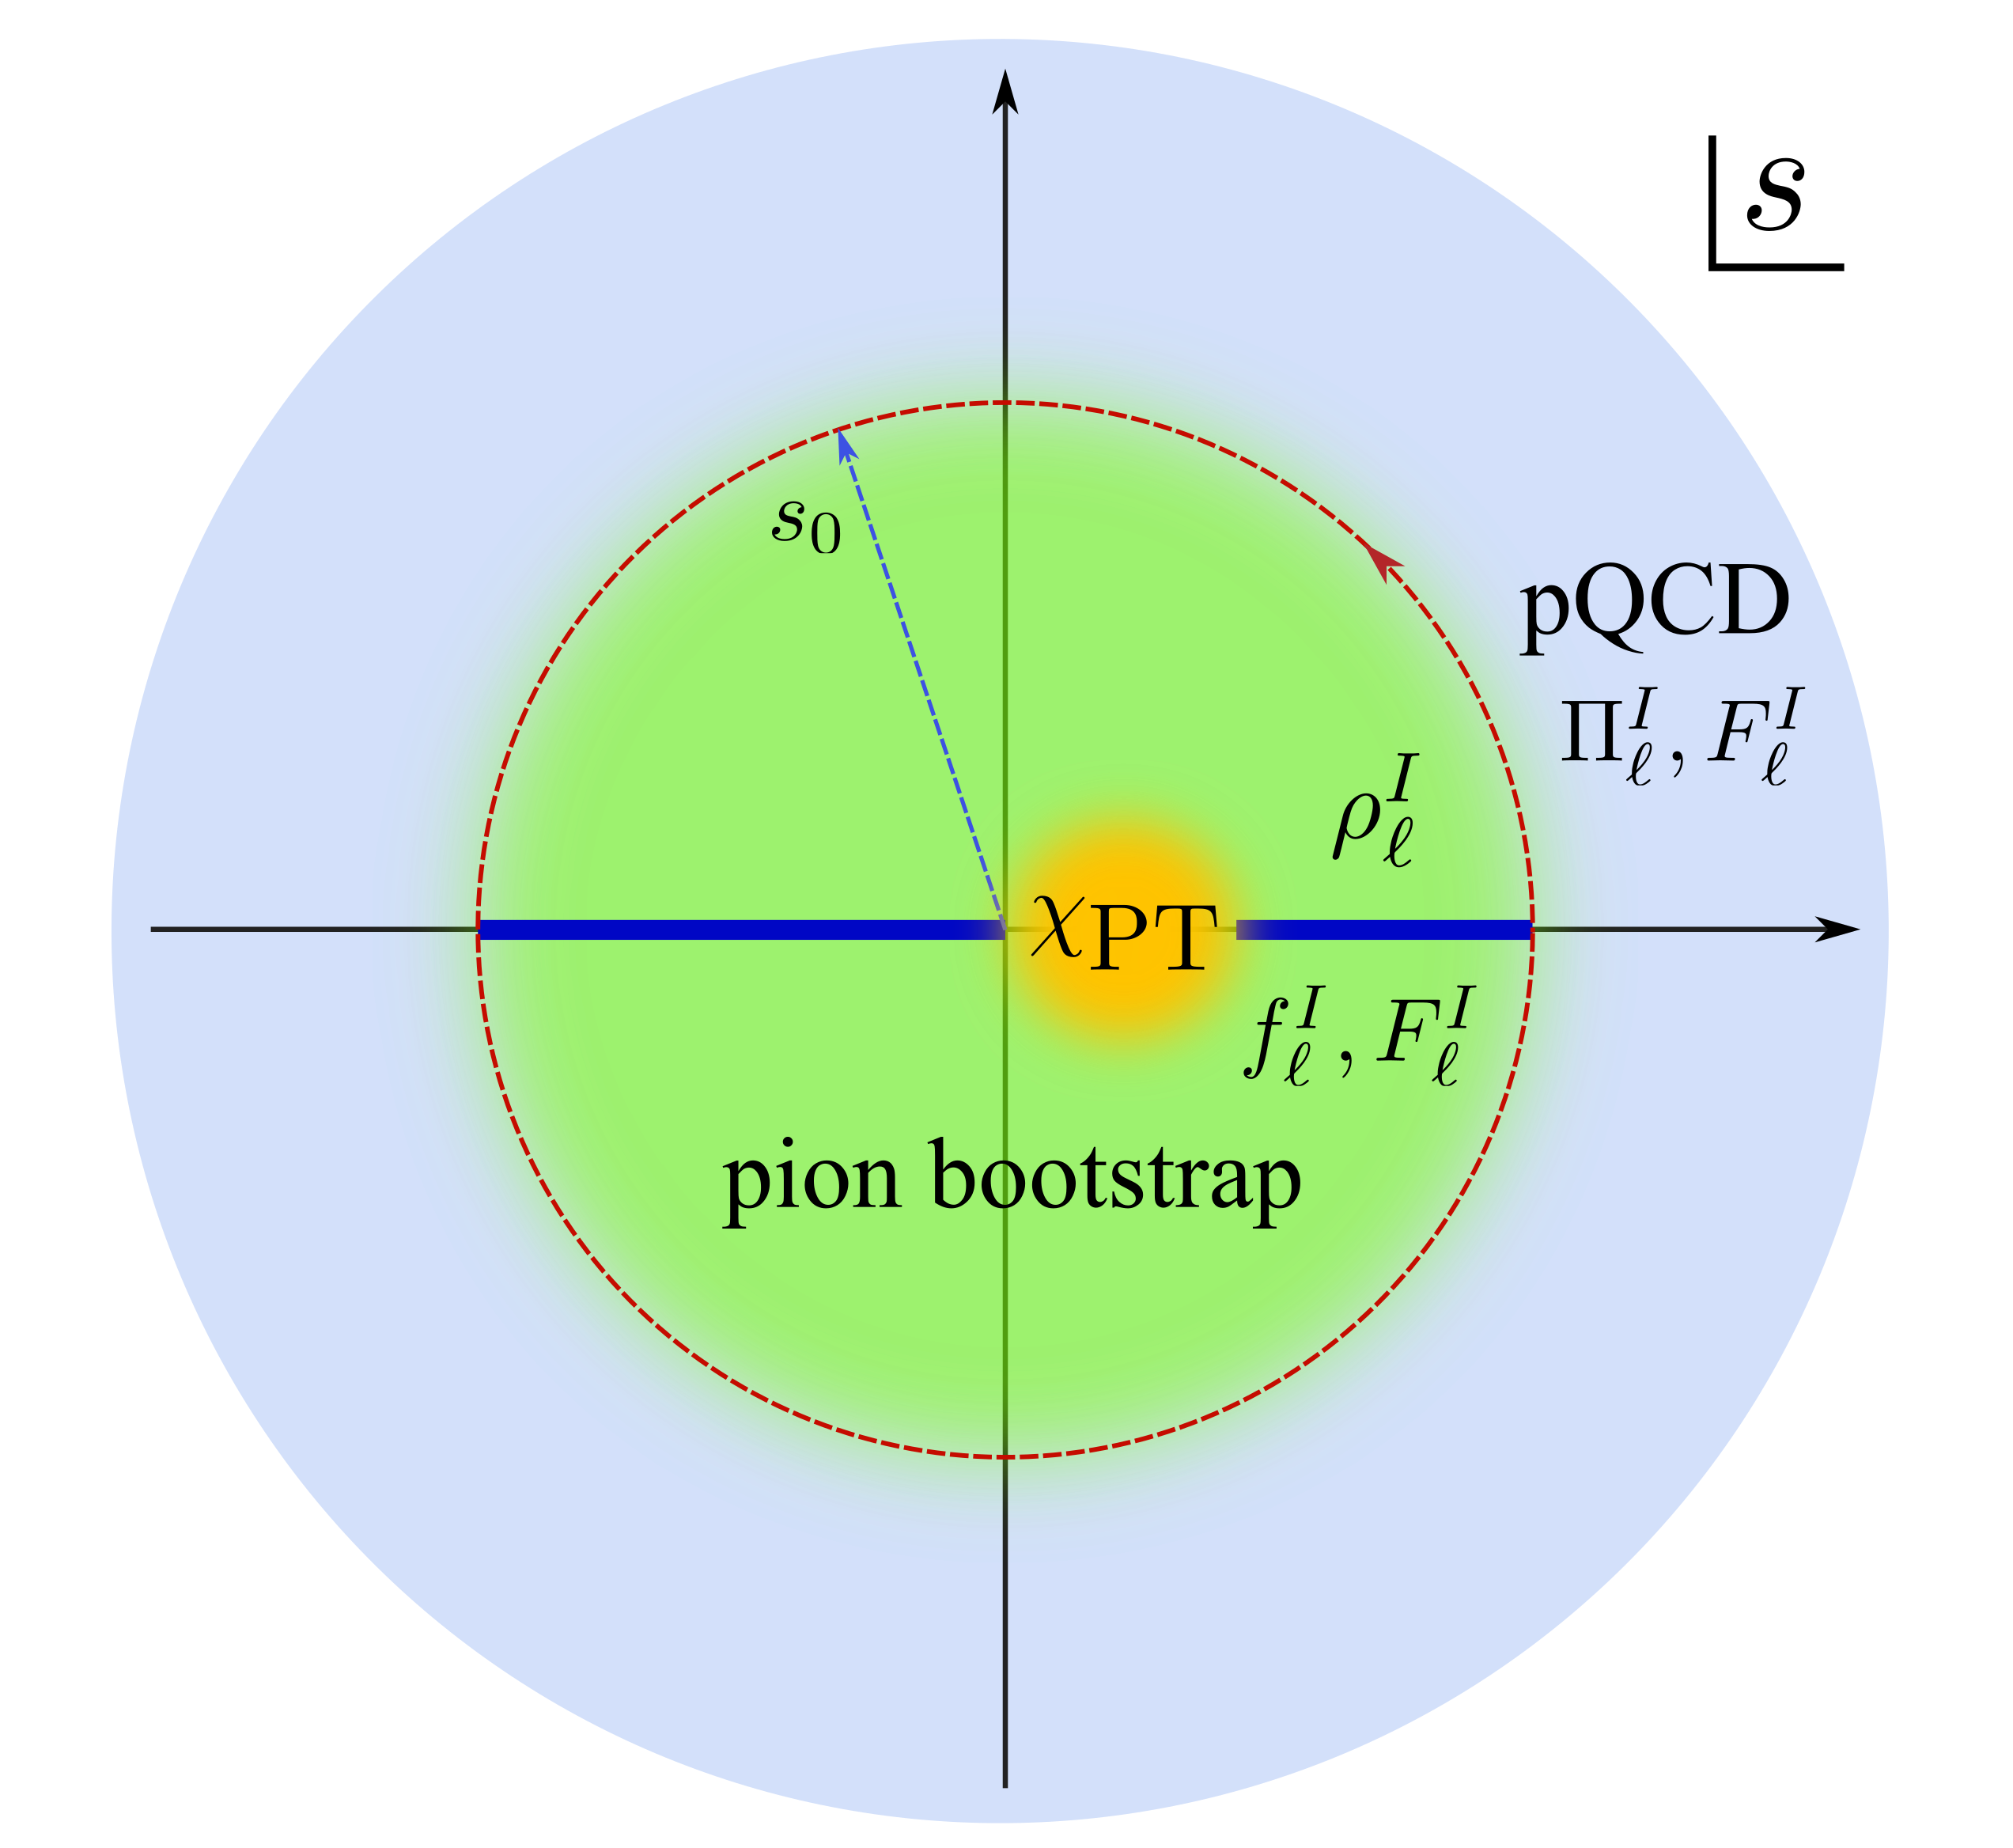
\includegraphics[width=.78\linewidth,height=78mm,keepaspectratio]{assets/original_method2.png}\end{center}
\src{[1] Fig.1，PDF 第5页，原始资产 method2.png。}
论文检验的核心思想是：低能手征信息约束 pion 散射的 IR 行为；电流的形状因子与相关函数把同一个 S 矩阵连接到高能 pQCD／SVZ 求和规则，进而在中间能区产生 QCD 特征。它不是对实验相移作多参数拟合，也没有证明一个唯一的完整 QCD 振幅。

\begin{tabularx}{\linewidth}{@{}p{12mm}p{45mm}Y@{}}\toprule
阶段&物理工作&主要论文输出\\\midrule
A&定义共同振幅、核、单位与约束&所有图的底层模型\\
B&纯散射与手征允许区域&Fig.3、Fig.4\\
C&锁定完整 IR 振幅并考察阈下／相移&Fig.5、Fig.6、Fig.7\\
D&FF／电流 Gram 与 QCD 信息联立&Fig.8--10 的共同基础\\
E&比较 UV 收缩、预选三点并求相移&Fig.8、Fig.9、Fig.10\\
F&按原文五组 \(M,L\) 比较分辨率&Fig.11\\\bottomrule
\end{tabularx}

\boxnote{teal}{\textbf{核心比较链：}同一有限散射设置下，先展示“只有 IR 输入”的对照，再加入 UV 约束并检查代表振幅。区域上的两个坐标不能代替完整系数；相移必须由保存的同一完整解恢复。}
\textbf{解耦原则：}Fig.3 是基线旁路；电流算子准备可以独立进行。C 的局部上边界选点不必等待 B3 所有方向细化。D 的共同可行见证也不等于 E 的全空间支持最优点。

\Ppage{18 步状态与主张判定}{status}{实现完成、数值证据和物理主张分别汇报；不使用一个总体完成百分比}
{\small
\begin{tabularx}{\linewidth}{@{}p{9mm}p{31mm}Yp{20mm}@{}}\toprule
步骤&对应任务&当前可支持的结论与边界&判定\\\midrule
A1&振幅与函数族&PV 交叉／同位旋参数化已实现；原 producer 身份未完整恢复。&\partialstatus\\
A2&手征／UV 输入&范数、单位、截止明确；SR 误差尺度、\(m_q\)、\(B\) 仍有执行选择。&\partialstatus\\
A3&算子与一致求值&原 H 与独立数学检查完成；无 PV 物理离节点定义。&\partialstatus\\
B1&有效有限支持&原式 primal/dual 及停止逻辑修正已实现。&\ok\\
B2&Fig.3 pure 区域&38 份支持，二维几何预算通过；不声称原图完全同一。&\ok\\
B3&Fig.4 六 \(\epsilon_\chi\)&包含／排除及严格缩小有证据；六域整体 .01 精度未完成。&\openq\\
C1&Fig.5 阈下曲线&三色线性改善与 S0 零点趋势得到支持。&\ok\\
C2&Fig.6 代表振幅&保存并原样复用绿色 3876 系数，选点不看相位。&\ok\\
C3&Fig.7 IR 相移&S0/S2 低能趋势及 P1 不足得到支持；仍有定量差异。&\partialstatus\\
D1&FF／电流 Gram&同一 S 与电流算子接线、100 个原 Gram 已验回。&\ok\\
D2&FESR／高能 FF&四矩及平方 FF 界实现；输入解释明确但不是唯一原设置。&\partialstatus\\
D3&共同可行点&完整 4076 维新模型见证通过；仅证明存在性。&\ok\\
E1&Fig.8 区域收缩&右端及上下两侧严格收缩；强非对称未复现。&\partialstatus\\
E2&预定三代表点&三点完整支持达标，完整向量在相位前固定。&\ok\\
E3&Fig.9--10／\(\eta\)&三点均有 P1 上穿；稳健性、部分弹性和 S0 形态不匹配。&\partialstatus\\
F1&Fig.11 五配置&四组通过；\((50,12)\) 尚无新联合见证。&\openq\\
F2&分辨率与原式&四组通过，三个 M 齐全；不是全部稳定性主张通过。&\partialstatus\\
F3&图谱与证据&原图／复现与来源可查；F 必须标注 partial。&\partialstatus\\\bottomrule
\end{tabularx}}
\boxnote{amber}{“支持／通过”仅指表中明确的有限或局部主张；不意味着原论文全部数值设置、连续性质或完整振幅身份已恢复。}
\src{[2] STATUS.md；[3] PAPER\_MAINLINE.json；[4--10] 各阶段当前结果。}

\Ppage{A：共同振幅与固定归一化}{amp}{论文 Eqs.(2.7)--(2.12)；所有 C/E/F 相位共用同一约定}
以 \(m_\pi=1\) 为单位，\(s+t+u=4\)。色散表示保留常数、两种单谱密度以及两种双谱密度：
\begin{align*}
A(s,t,u)={}&T_0+\frac1\pi\int_4^\infty dx
\left[\frac{\sigma_1(x)}{x-s}+\frac{\sigma_2(x)}{x-t}+\frac{\sigma_2(x)}{x-u}\right]\\
&+\frac1{\pi^2}\int_4^\infty dx\,dy
\left[\frac{\rho_1(x,y)}{(x-s)(y-t)}
+\frac{\rho_1(x,y)}{(x-s)(y-u)}
+\frac{\rho_2(x,y)}{(x-t)(y-u)}\right].
\end{align*}
\(\rho_2(x,y)=\rho_2(y,x)\)；一般不将 \(\rho_1\) 也强制对称。不同同位旋由同一 \(A\) 的交叉排列给出：
\[
\begin{split}
T^0&=3A(s,t,u)+A(t,s,u)+A(u,t,s),\\
T^1&=A(t,s,u)-A(u,t,s),\qquad T^2=A(t,s,u)+A(u,t,s).
\end{split}
\]
\[
f_\ell^I(s)=\frac14\int_{-1}^{1}P_\ell(z)T^I(s,t,u)\,dz,\qquad
S_\ell^I=1+i\kappa f_\ell^I,\quad \kappa=\pi\sqrt{1-\frac4s}.
\]

\begin{tabularx}{\linewidth}{@{}p{42mm}Y@{}}\toprule
约定&实现含义\\\midrule
偶／奇角动量&\(I=0,2\) 取偶 \(\ell\)；\(I=1\) 取奇 \(\ell\)。\\
\(L=10\)&每同位旋十个波：偶波 \(0,\ldots,18\)，奇波 \(1,\ldots,19\)。\\
目标平面&\(x=f_0^0(3),\,y=f_1^1(3)\)，是阈下投影坐标，不是截面。\\
变量总数&\(p=1+2M+M^2+M(M+1)/2\)；M50 为 3876。\\
联合原变量&加上两种 \(\operatorname{Im}F\) 与两种电流谱，共 \(p+4M=4076\)。\\\bottomrule
\end{tabularx}
\boxnote{teal}{\textbf{独立核对：}既有算子审计直接重建 Eq.(2.7) 的角投影，代表性 M50 行覆盖全部3876列，与生产行的最大差约 \(5.33\times10^{-15}\)。这支持归一化及接线一致，不证明所有程序错误已被排除。}
\src{[1] PDF 第9页；[11] OPERATOR\_AUDIT\_ZH.md；当前 kernels/operators/model/quotient。}

\Ppage{A：有限处方、密度界与方法差异}{finite}{当前生产只使用 PV 原生节点；未用 sine 的结论替代 PV 证明}
\[
\phi_j=\frac{\pi(j+1/2)}M,\qquad s_j=\frac4{\cos^2(\phi_j/2)},\qquad
w_j=\frac{s'_j}{M},\qquad
q_j(v)=\frac{w_jv}{s_j(s_j-v)}.
\]
当前 PV/midpoint 与解析 Legendre-\(Q\) 投影来自具名后续作者实现的公式映射，采用目标论文的中心 \(\nu_0=0\)。M50/L10 原 H 为 \(3011\times3876\)：3000个分波实／虚行、8个手征行、1个无穷远诊断行、2个目标行。

\boxnote{amber}{\textbf{定义域限制是实质问题：}PV 的物理值按节点 \(K+iI\) 指定，并非上式有理函数在其极点上的极限。目前定义了原生物理节点、阈下和阈值求值；其它物理离节点没有被定义。绘图连线不构成一个连续物理振幅。}

\textbf{当前正则化：}
\[
\|\rho_{\rm amp}\|_4\le B(M),\qquad
B(M)=100\!\left[M^2+\frac{M(M+1)}2\right].
\]
\(\rho_{\rm amp}\) 指实际双谱密度的独立条目，不含单谱 \(\sigma\)、\(T_0\) 或电流谱。当前 \(T_0\) 自由。M45/50/60 的 B 为 306000/377500/543000。该配方借鉴后续实现并在求值前固定，不是原文唯一指定的连续正则化范数。

\textbf{打包：}\code{C_flat} 中 \(\rho_2\) 对角为 \(\rho_{2,ii}\)，非对角为 \(2\rho_{2,ij}\)。L4 必须先还原实际密度；已核对不需要额外乘整体 \(\pi\) 或 2。

\begin{tabularx}{\linewidth}{@{}p{35mm}Y@{}}\toprule
保留／退休部分&科学边界\\\midrule
当前 PV 主线&全部系数保留；sampled/free；与后续核公式对应，但不等于找回2309原 producer。\\
有限 sine 历史&连续 Cauchy 变换、减法换元、T0／尾部／高spin必要条件及rank证据单独保存；执行已退休。\\
禁止的转移&不把 sine 的秩、可行性或无穷远必要条件自动加到 PV。跨 M 的密度运输只是初值，必须重新检查全部新约束。\\\bottomrule
\end{tabularx}
\src{[3,4,11] 当前合同、核映射、归一化审计；历史源码与证明输入保留。}

\Ppage{基本幺正性与证书的适用范围}{unitarity}{原生约束始终保留；弹性饱和不是新增硬条件}
全 S 矩阵幺正，投影到两 pion 弹性子空间后得到收缩条件。对每个保留分波：
\[
|S|\le1\quad\Longleftrightarrow\quad
\Delta=1-|S|^2=\kappa(2\,\operatorname{Im}f-\kappa|f|^2)\ge0
\quad\Longleftrightarrow\quad
\begin{pmatrix}1&S\\S^*&1\end{pmatrix}\succeq0.
\]
\(\operatorname{Im}f\ge0\) 本身不足够。阈值 \(s=4\) 且 \(f\) 有限时 \(S=1\)；阈下振幅不使用这一物理盘条件。允许 \(\eta<1\) 表示流向其它通道的概率，不能把它误报成违反幺正性。

\begin{tabularx}{\linewidth}{@{}p{39mm}Y@{}}\toprule
证据层级&本项目实际含义\\\midrule
实现／公式检查&独立角积分、解析阈值、正反幺正例、原复 Gram、OPE 矩与梯度／曲率控制。\\
原式可行性&保存完整原变量，检查全部列定盘、χ、L4、电流 Gram 主子式、FESR、FF。\\
支持最优性&原问题可行目标给下界，合法对偶给上界；不使用求解器标签替代。\\
新原生求值&用新的高精度核检查保存振幅，不只重复读取旧 H 的可行标记。\\
连续／完整物理性质&仍未证明全部能量、无限高自旋或完整连续 S 矩阵；有限检查不能升级为此结论。\\\bottomrule
\end{tabularx}

\boxnote{teal}{\textbf{当前具体结果：}新M50 tip的1500个原生分波重新生成后，幺正盘全部通过。十模块重构后再执行同一检查，结果保持；联合原式支持区间也与重构前一致。}
\textbf{精度解释：}768-bit 控制的是运算精度，不等于768-bit物理准确度。对保存 float64 H 的 Arb 界不含离散化、未知插值、输入处方及连续域误差。极小正裕量不能当作统一的物理误差条。
\src{[11] core10\_joint\_audit、core10\_fresh\_native；[2] SCIENCE；[1] Eqs.(2.9)--(2.12),(3.71)。}

\Ppage{B：手征约束及来源识别}{chiral}{原文说“某种范数”；当前选择有来源依据，但不假称原代码身份已恢复}
\[
\begin{split}
r_{01}(s)&=f_0^0(s)-\frac{3(2s-1)}{s-4}f_1^1(s),\\
r_{21}(s)&=f_0^2(s)-\frac{3(2-s)}{s-4}f_1^1(s).
\end{split}\qquad
s=\tfrac12,1,\tfrac32,2.
\]
约束的是\textbf{线性振幅残差}，不是直接取比值后再限制误差。当前将八个残差拼接为一个 Euclidean 球：
\[
\big\|(r_{01}(s_j),r_{21}(s_j))_{j=1}^4\big\|_2\le\epsilon_\chi.
\]
Weinberg 参照为
\[
(f_0^0,f_0^2,f_1^1)
=\frac{(2s-1,\;2-s,\;(s-4)/3)}{16\pi^2(f_\pi/m_\pi)^2},\quad
y=-x/15.
\]

\begin{tabularx}{\linewidth}{@{}p{23mm}YYY@{}}\toprule
原 Fig.5 曲线&\(\epsilon_\chi=.006\)&\(.004\)&\(.002\)\\\midrule
重建八维L2/\(\epsilon_\chi\)&1.000007&1.000020&1.000146\\\bottomrule
\end{tabularx}
从原图270个点重建四个χ位置的残差，三色均给出接近合并球边界的指纹；作者后续代码也明确使用 stack8。该依据先于本轮新相位；不是用实验 \(\rho\) 位置选择范数。源图插值误差保留，不能把上表略大于1当作原论文严格违例。

\[
K_{\rm combined}(\epsilon)\subseteq K_{\rm separate}(\epsilon)
\subseteq K_{\rm combined}(\sqrt2\,\epsilon).
\]
历史两个四维球的 primal 与 dual 均不能直接继承。当前166条旧手征查询经过新球的候选恢复／支持函数重验，并补必要方向；pure不受χ分组影响。

\boxnote{amber}{\textbf{尚未唯一恢复：}2309原始求解代码、密度正则化的精确定义与部分数值设置。源图指纹是有证据的执行推断，而不是完整 producer 的证明。}
\src{[4] CHIRAL\_SOURCE\_RESIDUALS、NORMALIZATION\_TRANSFER；[1] Eqs.(3.63)--(3.64)；[12] 作者后续代码。}

\Ppage{D：UV 输入与 FESR}{uv}{论文 Fig.2；连续关系到离散线性约束}
\begin{center}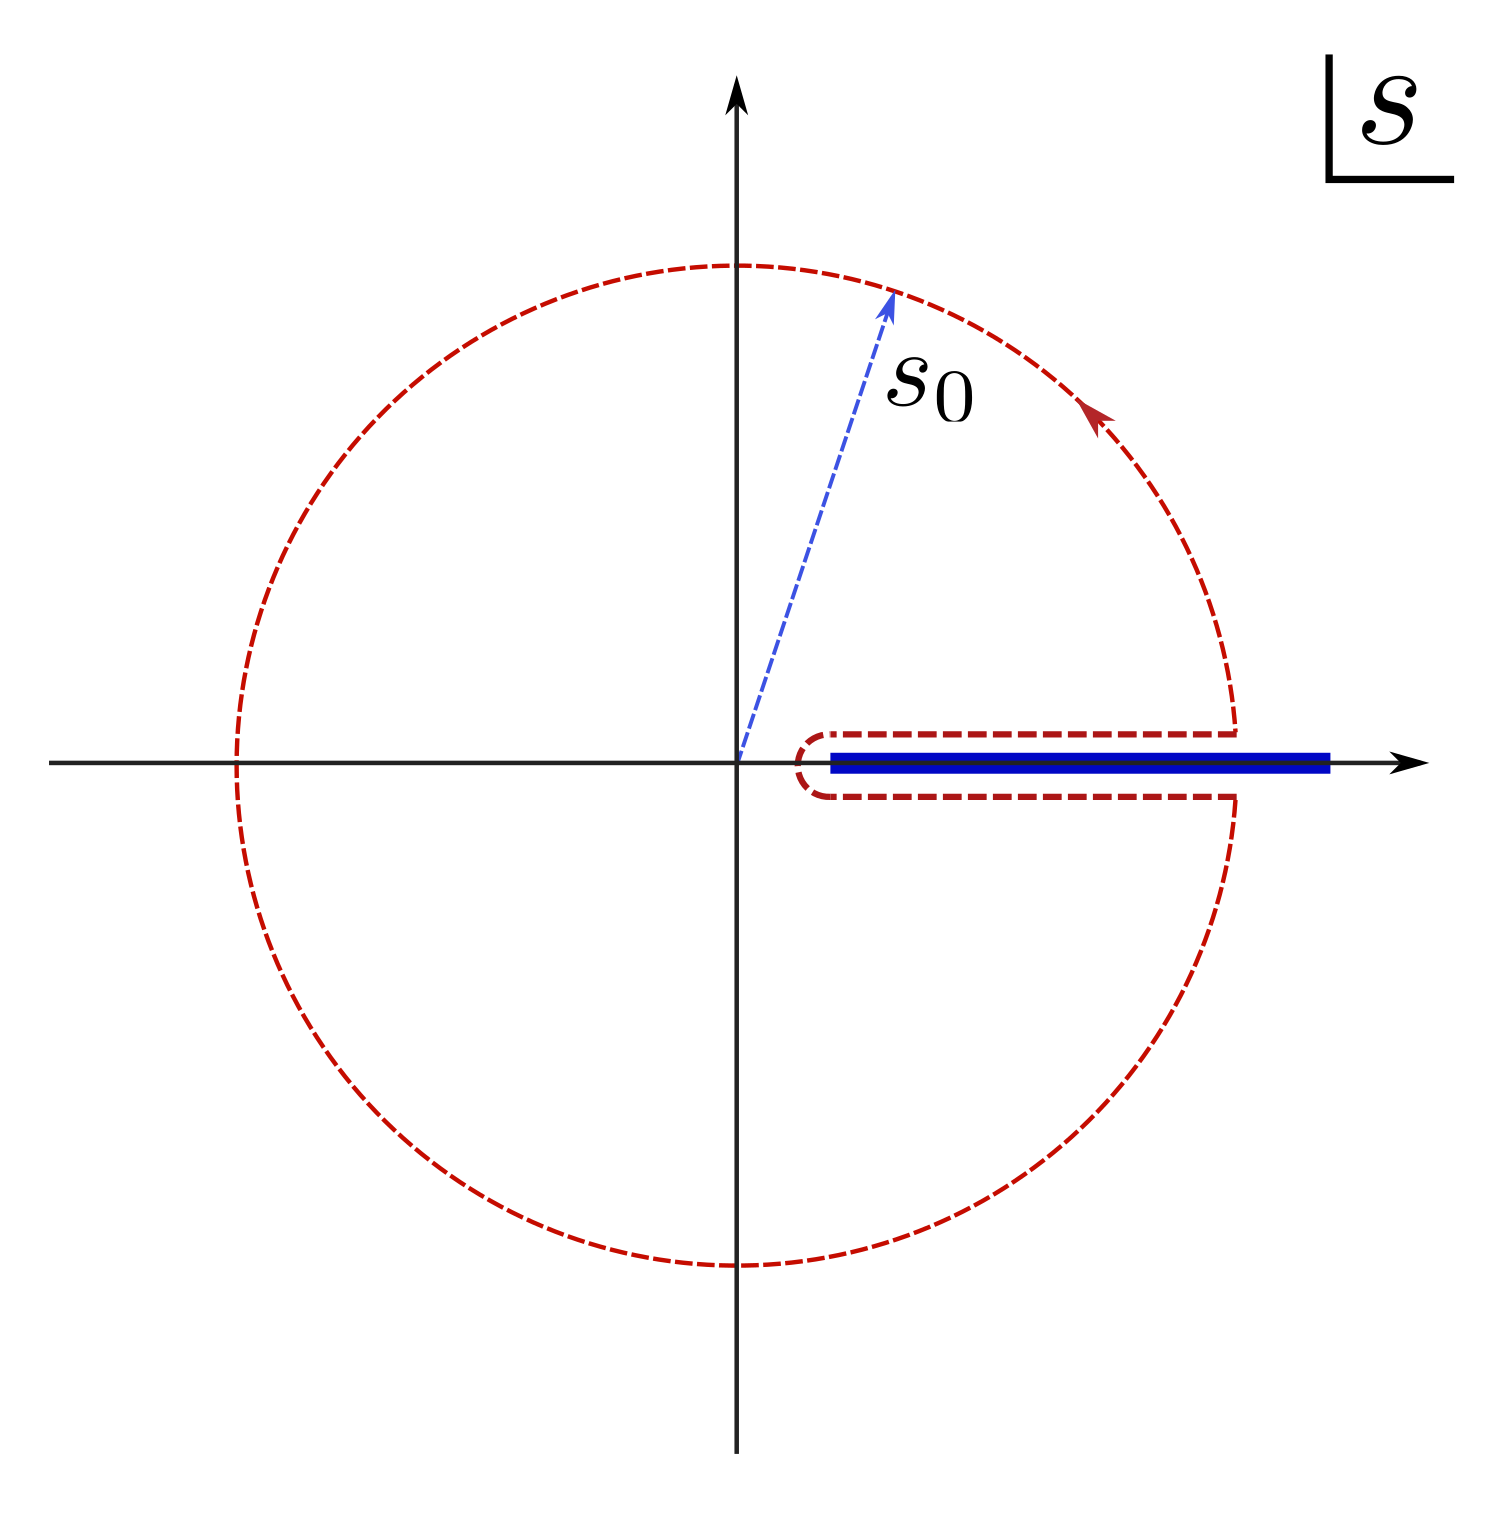
\includegraphics[width=.65\linewidth,height=65mm,keepaspectratio]{assets/original_FESR2.png}\end{center}
\src{[1] Fig.2，PDF 第17页，原始资产 FESR2.png。}
SVZ/OPE 在大圆上提供电流相关函数的信息，经 FESR 连接到低能谱积分。当前 S0 用 \(n=0,1\)，P1 用 \(n=-1,0\)：
\[
\int_4^{s_0}s^n\rho_{\rm cur}(s)\,ds
\ \longrightarrow\ \frac{\pi}{M}\sum_{s_i\le s_0}s'_i\,s_i^n\rho_{{\rm cur},i},
\qquad
s'_i=\frac{8\sin\phi_i}{(1+\cos\phi_i)^2}.
\]
当前按 Eq.(3.72) 的统一 \(\pi/M\) 权重及原生 \(s_i\le s_0\) 掩码使用 hard-midpoint；这不同于先前的 clipped-phi 端点单元修正。

{\small\begin{tabularx}{\linewidth}{@{}p{27mm}p{31mm}p{31mm}Y@{}}\toprule
通道／矩&当前raw目标&raw绝对误差&相对于目标的误差窗\\\midrule
S0，\(n=0\)&0.00238510421&0.002&约83.9\%\\
S0，\(n=1\)&0.111838139&0.002&约1.79\%\\
P1，\(n=-1\)&0.00422804571&0.002&约47.3\%\\
P1，\(n=0\)&0.145711207&0.002&约1.37\%\\\bottomrule
\end{tabularx}}
\boxnote{amber}{\textbf{关键来源不确定性：}原文误差公式写 raw 积分，打印 QCD 数值又带归一化。误差尺度／分组没有完整公开。raw 指以 \(m_\pi\) 计量、未除以 \(s_0^{n+2}\) 的矩；当前四个独立 raw 误差是声明的读法，不能称为已恢复的唯一作者实现，也不能因为相位不合预期就暗改为相对误差。}
\src{[1] Eqs.(2.50),(2.56),(3.72)--(3.75)；[3,4] 当前合同与截止决策。}

\Ppage{D：同一 S 的电流 Gram 与完整见证}{joint}{FF、谱与散射不能各自可行后就当作已联立}
\[
F_0(0)\simeq m_\pi^2=1,\quad F_1(0)=1,\quad
\operatorname{Re}F_i=1+K_{ij}\operatorname{Im}F_j,\quad \mathcal F=kF,
\]
\[
k_0^2=\frac{3\sqrt{1-4/s}}{256\pi^5},\qquad
k_1^2=\frac{(s-4)\sqrt{1-4/s}}{384\pi^5}.
\]
S0/P1 的每个节点共同施加原电流 Gram：
\[
G=\begin{pmatrix}
1&S&\mathcal F\\
S^*&1&\mathcal F^*\\
\mathcal F^*&\mathcal F&\rho_{\rm cur}
\end{pmatrix}\succeq0.
\]
这里的 S 必须来自与其它分波相同的完整振幅。电流谱与幅度双谱密度是不同变量。正对角合同变换／实基表示仅用于数值计算，最终检查原式。

\begin{tabularx}{\linewidth}{@{}p{47mm}Y@{}}\toprule
固定输入&当前值\\\midrule
\(m_\pi,f_\pi,\sqrt{s_0}\)&140 MeV，约92 MeV，1.2 GeV\\
\(N_c,N_f,\alpha_s\)&3，2，0.4\\
\(m_u,m_d\)&4 MeV，7.3 MeV；FF中的 \(m_q\) 用算术平均\\
凝聚&胶子 \(0.023\,{\rm GeV}^4\)；标量 \(-(.1\,{\rm GeV})^4\)\\
高能平方FF界&\(|\mathcal F_0|^2\le1.9544388\times10^{-7}\)，\(|\mathcal F_1|^2\le3\times10^{-5}\)，只在 \(s_i>s_0\)\\\bottomrule
\end{tabularx}
\boxnote{teal}{\textbf{D3 当前见证：}投影 \((x,y)\simeq(.07143138818,-.00455776509)\)，完整4076维；1500盘、χ、L4、100 Gram、四矩及14 FF全部通过。密度范数约357458.77，小于377500。}
以上FF界同样使用 \(m_\pi=1\) 与 \(\mathcal F=kF\) 的无量纲归一化。生成器是392个求解变量的父幅度凸包＋电流 SDP，51步、约0.553秒（求解器时间）。它输出合法完整见证，\textbf{不是}全空间支持最优点；受限搜索速度不与 E 全空间速度作排名。
\src{[7] D3\_paper\_hull；D1\_hard\_M50；[11] 原复Gram／OPE独立核对。}

\Ppage{求解器、原式支持与精度解释}{solver}{2309未明确指定具体solver；性能比较与科学问题定义分开}
2309 v3 数值正文没有明确指定 Newton、CVX 或 MOSEK；TeX 的 CVX 书目条目处于注释中。作者后续公开脚本明确使用 CVX 建模与 MOSEK 求解。[10,12] 当前仓库没有同一冻结问题、同一精度和硬件下的 MOSEK 基准，\textbf{不能宣称自编 Newton 更优}。

\textbf{当前求解路径}
\begin{enumerate}
\item B：保留全部有限振幅方向，使用可行障碍路径、QR预条件／长精度CG及原式支持验界。
\item D：Clarabel 在已知幅度凸包上寻找共同电流见证；或者用完整 Phase I 保持散射、χ、L4为硬约束，只对电流子系统引入辅助 \(\tau\)。
\item E/F：完整原变量对应的联合支持；从适当内点重新中心化，已完成中心按既有路径续接；使用可逆换元、正障碍权重及精确可行线搜索。
\end{enumerate}
\[
L=c^\top z_{\rm feasible}\ \le h_K(c)=\sup_{z\in K}c^\top z\ \le U,
\qquad \mathrm{gap}=U-L.
\]
上界在原 H／电流算子和合法对偶上核验；不以 Newton 减量、CG残差、AlmostSolved 或超时标签替代。相同验界也可以接受成熟求解器的输出，不是自编算法独有的优势。

\begin{tabularx}{\linewidth}{@{}p{41mm}Y@{}}\toprule
数值量&不能被误读为\\\midrule
方向目标 gap&每个系数或相移具有同量级误差；完整极值振幅唯一。\\
辅助 \(\tau>0\)&原联合可行；或原问题已被证明不可行。\\
当前网格通过&连续能区与无限高自旋均无违例。\\
高精度运算／79测试&恢复了原作者所有参数；原图或所有claims自动通过。\\\bottomrule
\end{tabularx}
\textbf{已修正的数值错误：}B 的停止逻辑曾忽视原目标支持误差；复用QR时实际线性残差曾约 .04。现要求质量不足则刷新／退出，并用原式上下界验收。失败分支和输入保留，不能据其失败贬低 MOSEK。
\src{[10] SOLVER\_DECISION、B\_SOLVER\_FIX；[11] 核心数学及重构验证。}

\Ppage{支持界为什么不依赖求解器标签}{supportmath}{B 的原式推导与 E/F 的扩展；数值改进不能改变可行集合}
令 \(Z_i=\kappa_i f_i\)。幺正盘等价于 \(|Z_i-i|\le1\)，因此对于任意实数 \(a_i,b_i\)，
\[
a_i\operatorname{Re}Z_i+b_i\operatorname{Im}Z_i
\le b_i+\sqrt{a_i^2+b_i^2}.
\]
把原目标写为盘线性项、八维手征残差 \(r_\chi\) 以及实际密度的余项：
\[
c^\top z=\sum_i\big(a_i\operatorname{Re}Z_i+
b_i\operatorname{Im}Z_i\big)+y^\top r_\chi+
r_\rho^\top\rho_{\rm amp}.
\]
这里必须先消去自由 \(T_0,\sigma_1,\sigma_2\) 方向的残差；当前验界通过原生行的解析校正实现，不能给自由方向凭空增加一个系数界。由 Cauchy--Schwarz 与 Hölder 不等式得到
\[
\boxed{\quad
h_K(c)\le
\sum_i\big(b_i+\sqrt{a_i^2+b_i^2}\big)
+\epsilon_\chi\|y\|_2+B\|r_\rho\|_{4/3}.
\quad}
\]
密度余项中的打包因子必须先转回实际 \(\rho\)。在 pure 情形去掉χ项；历史 separate-L2 则是两个对偶二范数之和，不能与当前合并范数混用。

\textbf{联合问题的扩展。}E/F 在上述原目标分解中加入电流 Gram 的半正定乘子、FESR／FF 乘子及仿射常数，并处理电流自由方向的余项。保存的完整可行点给出下界。只有两侧都合法，目标差才能作为支持验收依据。

\textbf{L4 障碍中的消元。}写 \(v_j=\rho_j/B\)，则
\[
\sum_jv_j^4\le1
\ \Longleftrightarrow\
\exists\,u_j\ge v_j^2,\qquad\sum_ju_j^2\le1.
\]
实现采用标准二阶锥提升的障碍，对辅助 \(u\) 的中心条件作消元，再以 Schur 补形成 Newton 曲率。消掉的是辅助变量，所有物理密度方向仍保留；不能用删除小奇异值方向来声称原问题更容易。

\boxnote{amber}{原式界针对保存的有限算子，仍不包含未知处方、连续延拓与离散化误差。成熟锥求解器或自编 Newton 都应接受同一个原式验收，而不是靠 solver 名称保证科学正确。}
\src{当前 imaginary.support\_outer、quotient.barrier\_terms；[10,11] 支持与曲率审计。}

\Ppage{B2／Fig.3：纯 S 矩阵基线}{fig3}{仅基本散射条件；论文明确该图后续不再直接使用}
\begin{center}{\bfseries 论文原图 Fig.3}\\[1mm]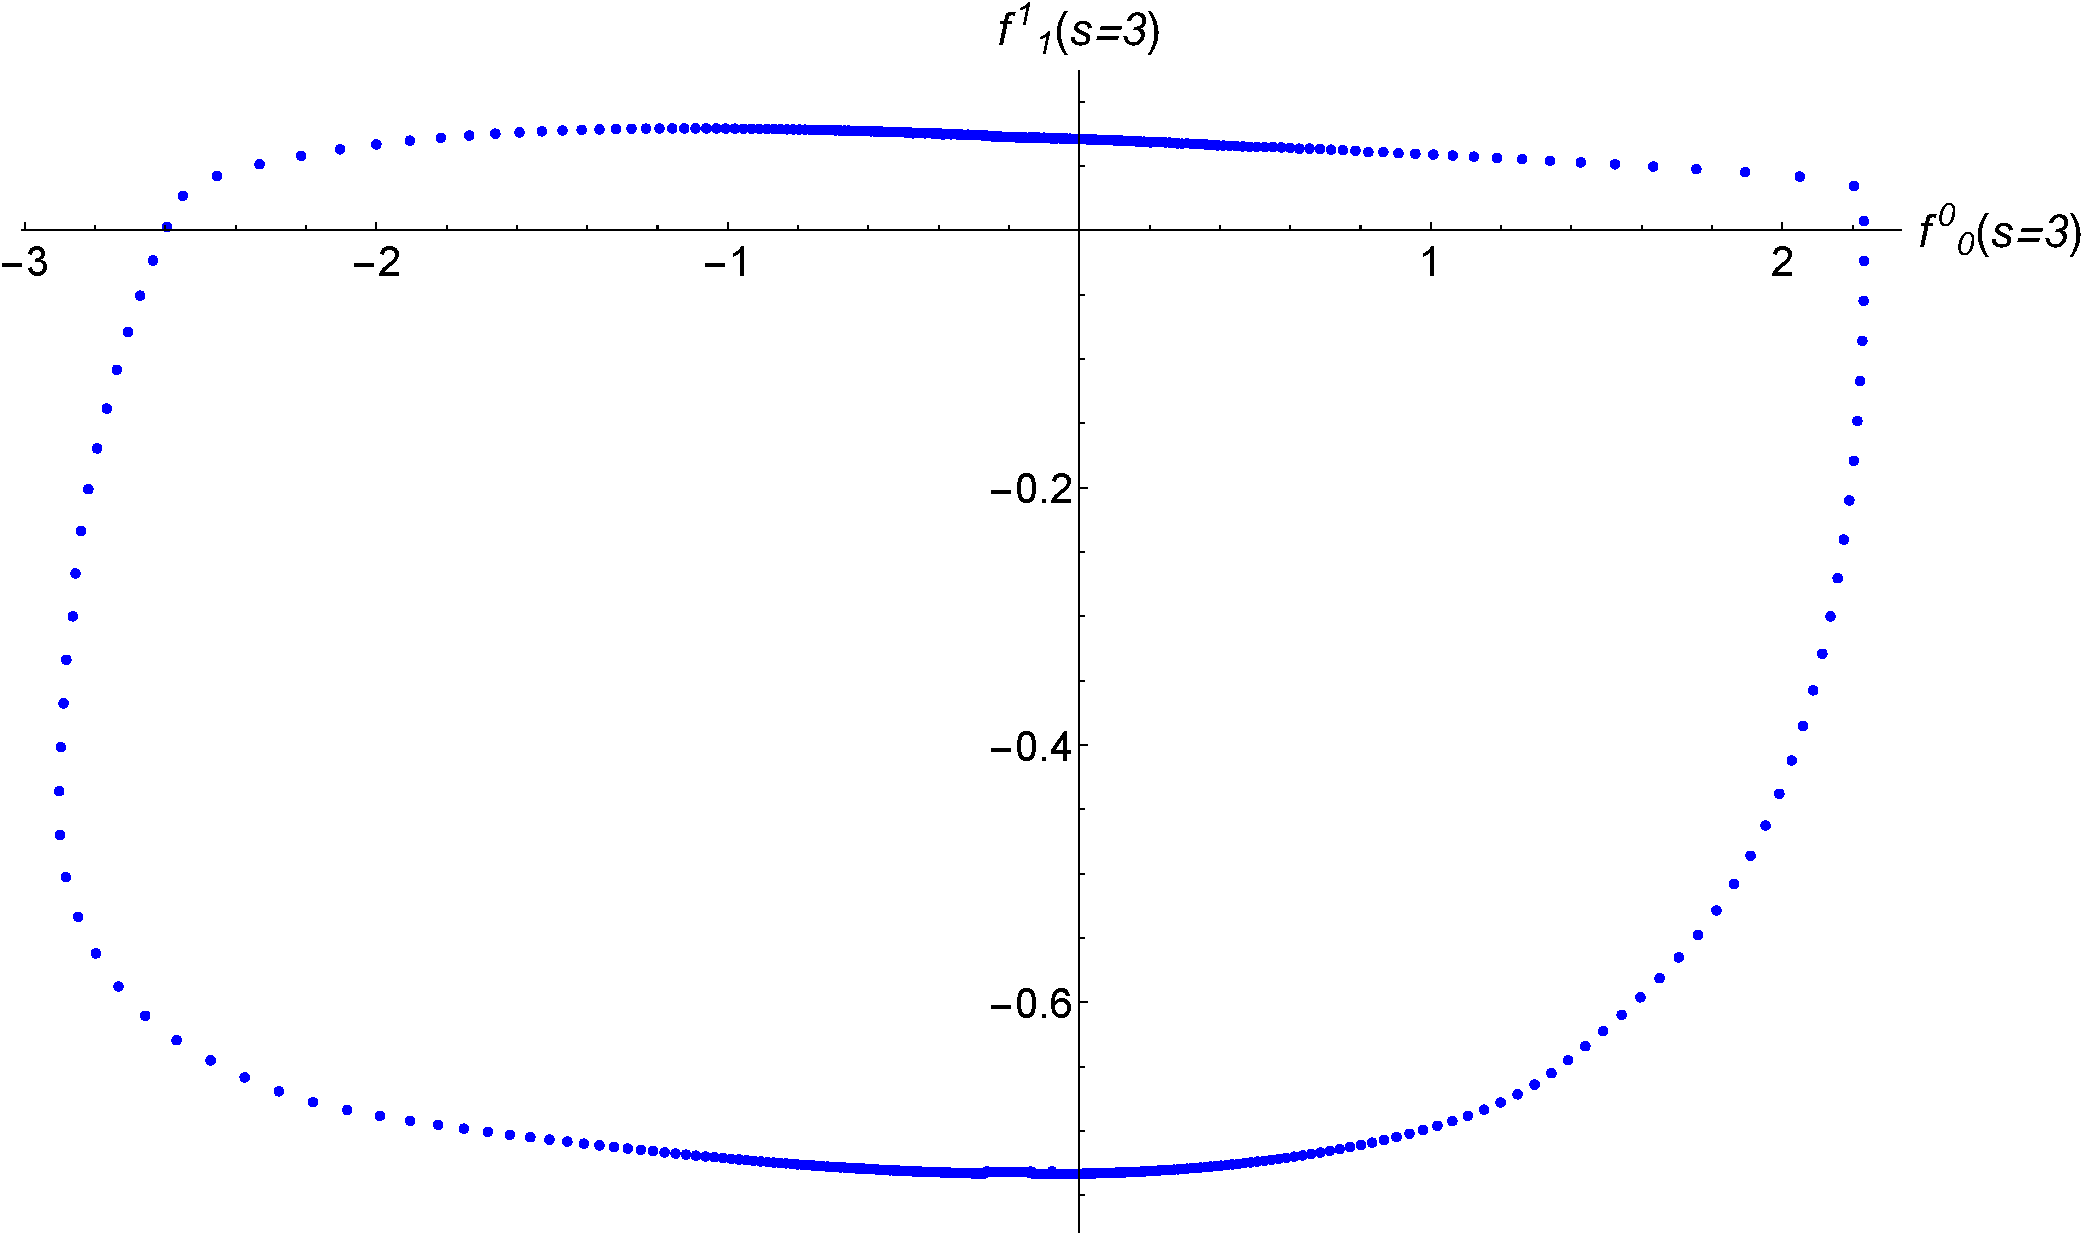
\includegraphics[width=.84\linewidth]{assets/original_purSplot.pdf}\end{center}
\begin{center}{\bfseries 当前有限模型：内包与合法外界}\\[1mm]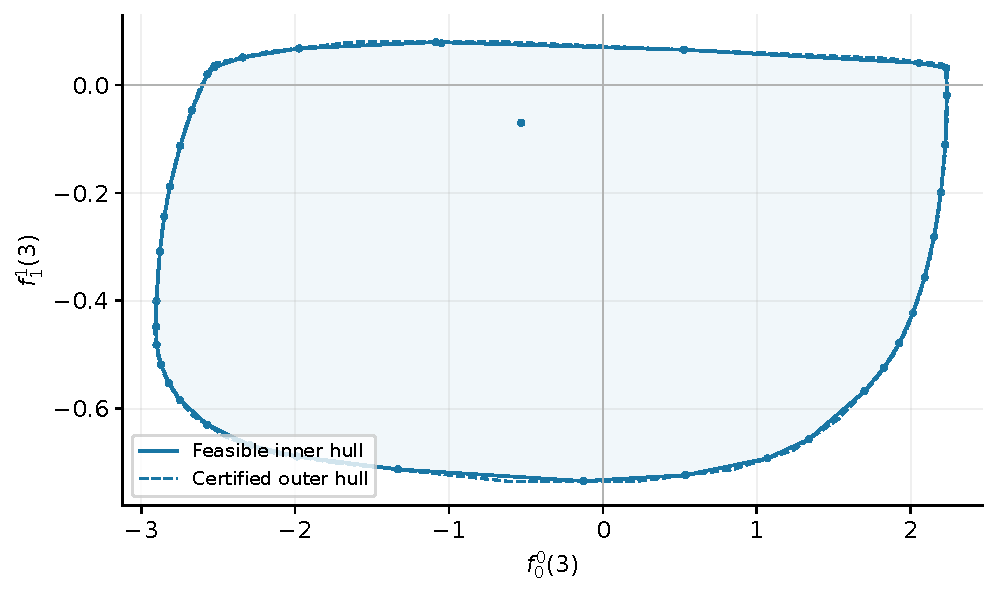
\includegraphics[width=.84\linewidth]{assets/ours_fig3.pdf}\end{center}
\boxnote{teal}{\textbf{当前证据：}同一 PV/M50/L10、自由 \(T_0\)、B=377500 下，38份合法支持构成 pure 区域。内外包距离上界 .00967577335，满足预声明 .01 预算。}
\textbf{判定：}有限基线与区域构造得到支持；外形相似不等于原 producer 身份已恢复。这里的距离度量是 \(q=(x,y)\)，与手征图的缩放度量不同。
\src{[1] Fig.3，PDF 第27页；[5] regions\_IR\_lower\_003 中 mode=pure；新图仅重绘保存的顶点。}

\Ppage{B3／Fig.4：六种手征容差的区域}{fig4}{原图只显示 \(x\ge0\)；实线为本方可行内包，虚线为有效外包}
\begin{center}{\bfseries 论文原图 Fig.4}\\[1mm]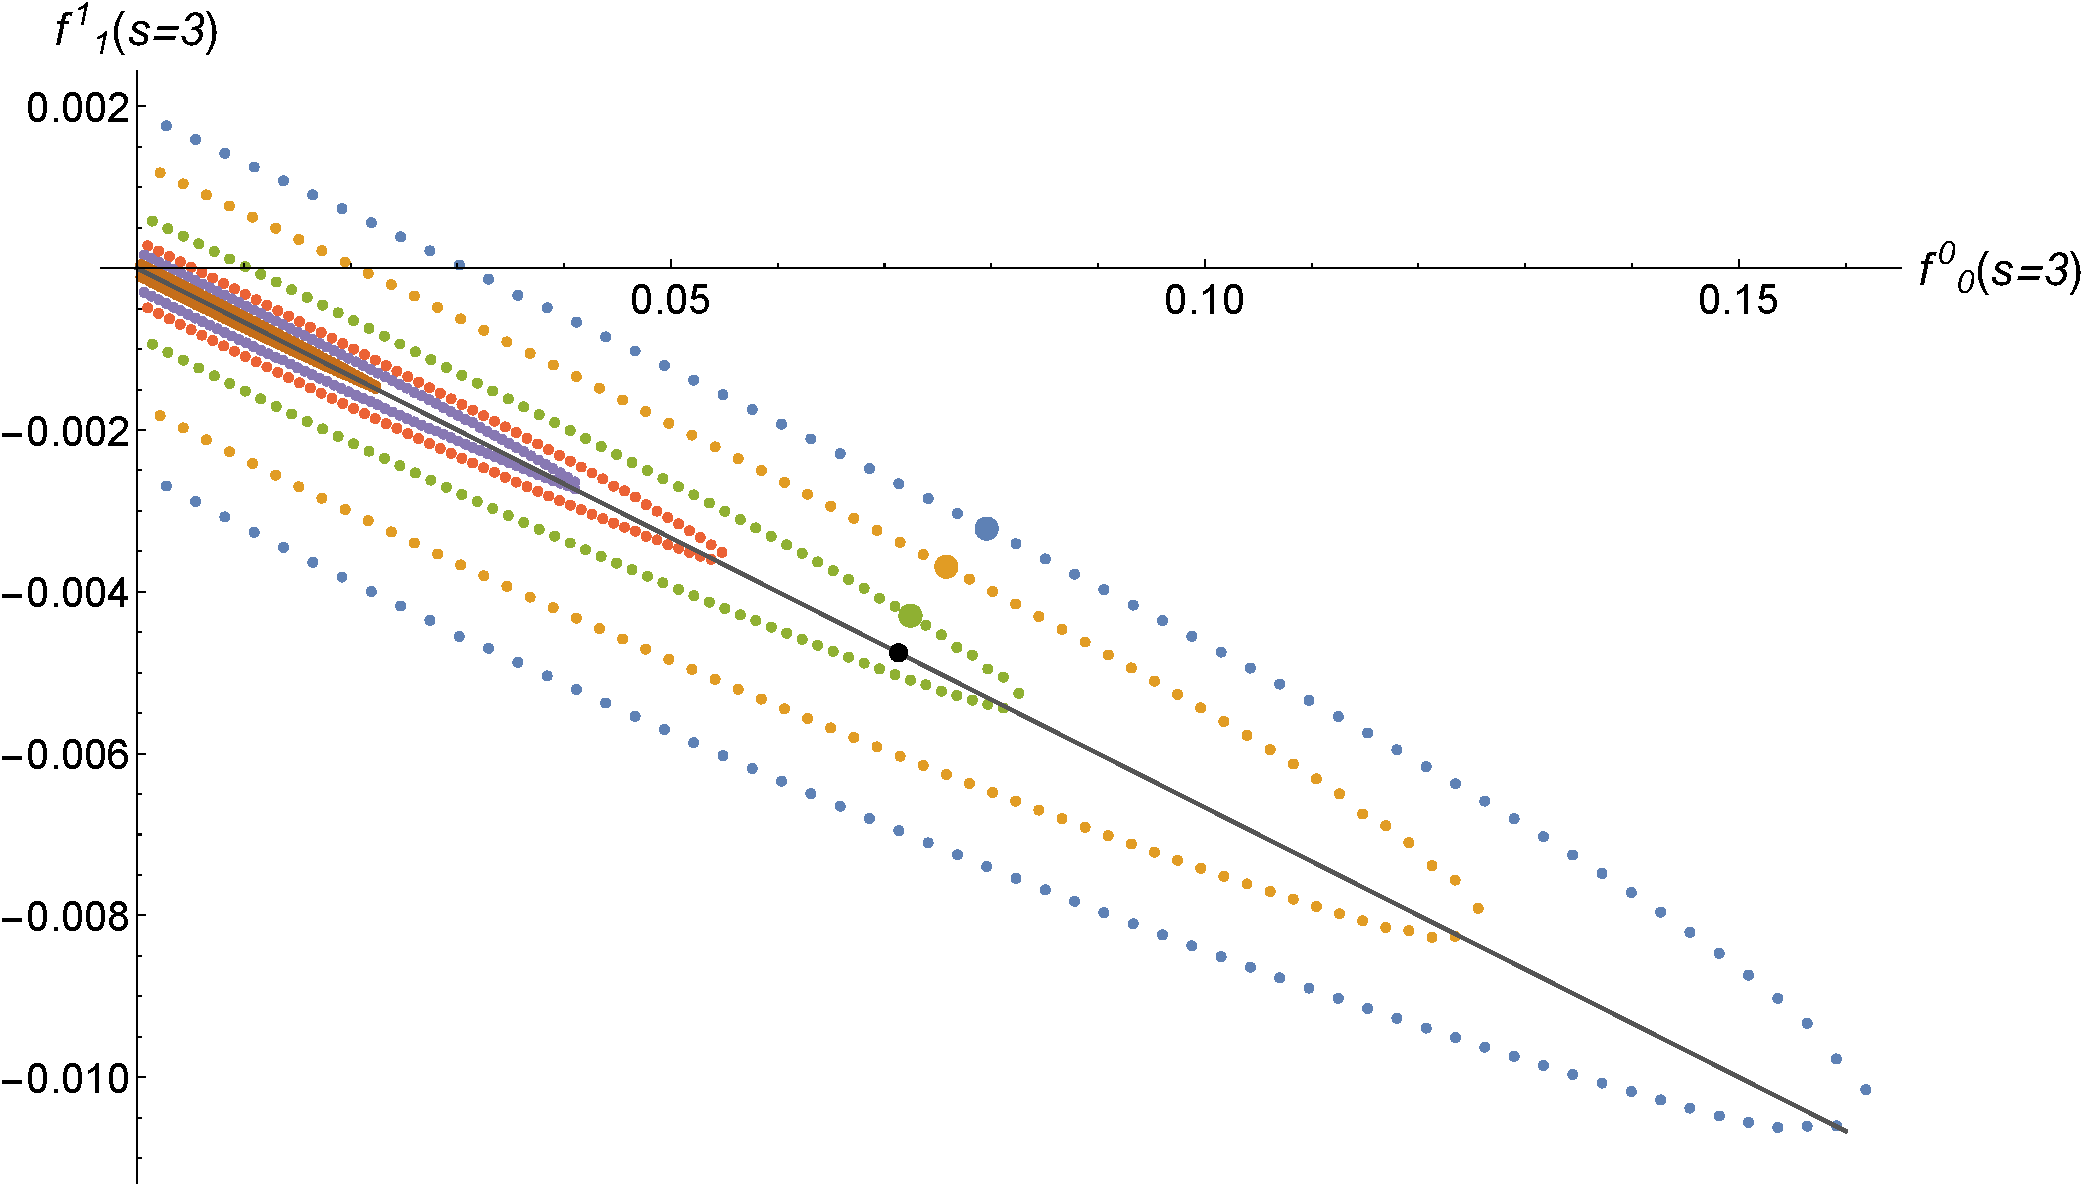
\includegraphics[width=.96\linewidth]{assets/original_chiplot.pdf}\end{center}
\begin{center}{\bfseries 当前 combined-L2 模型}\\[1mm]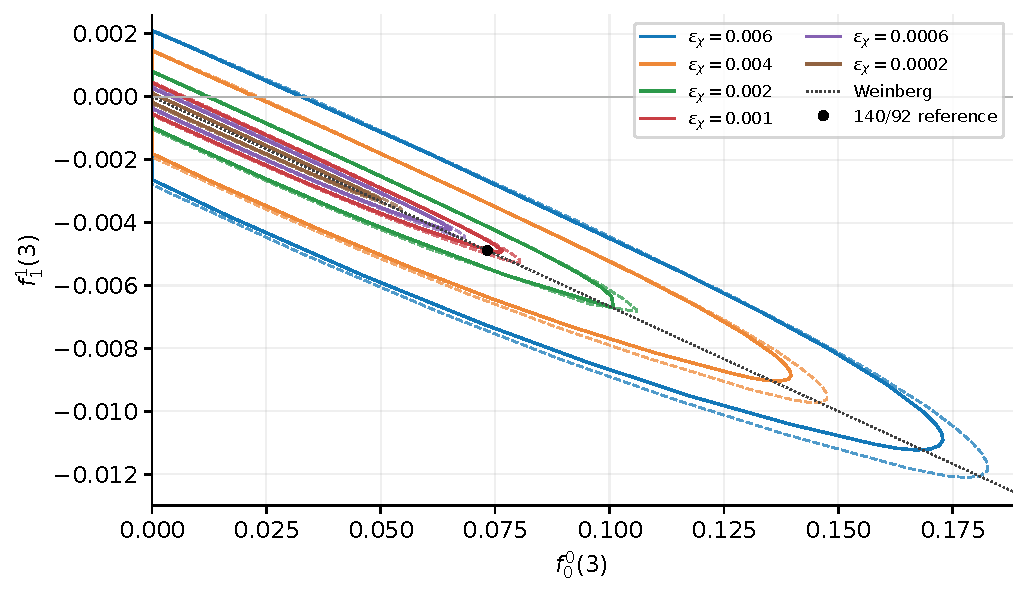
\includegraphics[width=.96\linewidth]{assets/ours_fig4.pdf}\end{center}
\boxnote{amber}{\textbf{支持：}容差减小使集合嵌套、右端严格缩小；较小容差可排除物理参考点。\\
\textbf{未闭合：}六个区域的整体几何精度尚未达到 .01；原图与本模型的定量范围也不一致。}
\src{[1] Fig.4，PDF 第28页；[5] FIG4\_CORE\_CLAIMS、当前212条合格记录的区域汇总。颜色／图轴分别以各图图例为准。}

\Ppage{Fig.4：哪些结论已经确定}{bquant}{几何精度不足与模型／原图差异不是同一个问题}
手征区域的距离预算使用
\[
q=\left(\frac{x}{x_{\rm ref}},\,\frac{y+x/15}{\epsilon_\chi}\right),\qquad
x_{\rm ref}=\frac5{16\pi^2(92/140)^2}\simeq.07332139.
\]
.01 不是对两个原始坐标统一施加的绝对误差。

{\small\begin{tabularx}{\linewidth}{@{}p{15mm}p{48mm}p{32mm}Y@{}}\toprule
\(\epsilon_\chi\)&当前右端支持区间&原图最大显示 \(x\)&整体距离上界\\\midrule
.006&[.17287099,.18256775]&.16188036&.14207359\\
.004&[.13967614,.14753914]&.12559519&.11679601\\
.002&[.10084542,.10594017]&.08257301&.07372583\\
.001&[.07652356,.08032184]&.05478209&.07443163\\
.0006&[.06528726,.06832086]&.04100125&.08859216\\
.0002&[.04998082,.05452031]&.02236258&.22661593\\\bottomrule
\end{tabularx}}
相邻右端区间严格分离，故“随容差下降而严格缩小”有原式证据。六组都已经存在超过原图最大显示 \(x\) 的合法内点，继续收紧同一模型的外界不能删除这些点。原图显示最大值不是作者的严格支持上界，因此这不是对论文的反证。

\begin{tabularx}{\linewidth}{@{}p{29mm}YY@{}}\toprule
容差&公式140/92参考点&原Fig.4黑点读数\\\midrule
.006 / .004 / .002&已证包含&已证包含\\
.001&\textcolor{red}{未决}&已证包含\\
.0006 / .0002&已证排除&已证排除\\\bottomrule
\end{tabularx}
包含由完整可行振幅的正权凸组合证明，排除由有效支持平面证明。

原黑点读数约 \((.07131334,\allowbreak-.00475418)\)，不能与公式点混用。论文选 .002 还结合 Fig.5 的阈下线性行为，并不由这张包含表证明其唯一性。
\src{[5] FIG4\_CORE\_CLAIMS.json/.md，regions\_IR\_lower\_003；源图显示读数不是统计置信区间。}

\Ppage{C1／Fig.5：阈下三波逐面板对照}{fig5}{三种 \(\epsilon_\chi\)，相同预定物理 \(x_{\rm ref}\) 的上侧代表振幅}
\pairfig{original_lin1.pdf}{ours_fig5_S0.pdf}{5(a)：S0}
\vspace{3mm}
\pairfig{original_lin2.pdf}{ours_fig5_S2.pdf}{5(b)：S2}
\vspace{3mm}
\pairfig{original_lin3.pdf}{ours_fig5_P1.pdf}{5(c)：P1}
\boxnote{teal}{随着 \(\epsilon_\chi\) 减小，三波对 Weinberg 线性式的偏离均减小；蓝色未见S0零点，橙／绿零点向 \(s=.5\) 靠近。这支持论文的阈下比较主线。}
\src{[1] Fig.5，PDF 第29页；[6] C1\_fig5/profiles.json，81个阈下点。右图是既有数据重新排版，无新求解。}

\Ppage{C1--C2：线性改善与 Fig.6 的同一振幅}{fig6}{原图的“靠近黑点”不是一个已公开的唯一精确距离最小化规则}
\pairfig{original_chiplot2.pdf}{ours_fig6.pdf}{6}
\src{[1] Fig.6，PDF 第30页；[6] C2\_fig6 的完整系数及 selection。右图虚线外包的宽度仍反映 B3 未完成精度。}

{\small\begin{tabularx}{\linewidth}{@{}p{18mm}YYYp{26mm}@{}}\toprule
\(\epsilon_\chi\)&S0 最大线性偏离&S2 最大线性偏离&P1 最大线性偏离&S0 零点括区\\\midrule
.006&.0665273&.0108100&.00341742&所查网格未见\\
.004&.0373882&.00726071&.00223707&[.30,.35]\\
.002&.0199366&.00414252&.00111497&[.40,.45]\\\bottomrule
\end{tabularx}}

\textbf{C 的局部边界证据。}对任意有效上侧支持平面 \(n_xx+n_yy\le U\)、\(n_y>0\)，以及已验完整点 \((x_c,y_c)\)：
\[
0\le y_{\max}(x_c)-y_c
\le\frac{U-n_xx_c}{n_y}-y_c.
\]
三色的上侧距离／\(\epsilon_\chi\) 分别为 .00684087/.00143989/.00698352，均满足同一 .01 局部预算。它可使 C 独立推进，\textbf{不等于}B3 全区域精度已经通过。

\boxnote{teal}{C2 原样保存 C1 绿色的全部3876系数；C3 使用的仍是这个向量。没有看到相移后重新挑点或混合振幅。对应的是预声明几何角色，不是已恢复的原作者完整向量。}
\src{[6] C\_RESULT、C\_LOCAL\_SELECTION；线性偏离是本方采样极值，零点是采样括区。}

\Ppage{C3／Fig.7：只有 IR 输入的相移}{fig7}{每个面板左为论文原图，右为同一个绿色完整振幅}
\pairfig{original_chiS0plot.pdf}{ours_fig7_S0.pdf}{7(a)：S0}
\vspace{3mm}
\pairfig{original_chiS2plot.pdf}{ours_fig7_S2.pdf}{7(b)：S2}
\vspace{3mm}
\pairfig{original_chiP1plot.pdf}{ours_fig7_P1.pdf}{7(c)：P1}
\boxnote{teal}{本方 IR-only 的 P1 到1.2 GeV仅约 \(8.64^\circ\)，未出现目标 \(\rho\) 上穿；S0/S2低能形态较接近。支持“只用这些IR信息不足”的示例比较，不证明整个IR可行集都不能有共振。}
\src{[1] Fig.7，PDF 第31页；[6] C3\_fig7、C3\_evaluate；43原生节点加阈值、132项检查通过。灰色为原图中的现象学／实验参考。}

\Ppage{C：原图误差、对照逻辑与解释边界}{cquant}{区分与“论文bootstrap曲线”比较、与“实验／现象学”比较}
\begin{tabularx}{\linewidth}{@{}p{62mm}YYY@{}}\toprule
相移 RMS 差（度）&S0&S2&P1\\\midrule
对原Fig.7 bootstrap，同原生 \(s\)&5.5595&0.5039&2.7422\\
对现象学曲线，公共GeV范围&7.3549&2.0329&85.6347\\\bottomrule
\end{tabularx}
P1 与原论文的 IR-only 曲线较接近，并不意味着与真实 \(\rho\) 共振相符；两种对照给出不同答案。上述RMS为曲线读数差，不是 \(\chi^2\)、实验误差或置信区间。

\textbf{原生坐标对照。}原图能量标记反推的显示质量约139.57 MeV，与正文140 MeV略有差别。当前比较同时保存原GeV坐标和同一个无量纲原生 \(s\) 的结果；映射由横坐标识别，不调整生产 \(m_\pi\)，也不以相位拟合求映射。

\textbf{C 到 E 的比较是什么？}
\begin{itemize}
\item 保持散射 H、χ范数与容差、B和基本幺正性相同；UV侧增加同一S的电流／FF／FESR条件。
\item IR与UV分别按预声明的几何规则选择完整代表振幅；不是同一个不变振幅在加入约束后“改变相位”。
\item IR示例P1不合理、UV示例P1有共振，是对方法机制的正面证据；不自动证明所有UV解都正确、所有IR解都错误。
\end{itemize}

\boxnote{amber}{\textbf{C 仍保留的差异：}S0中／高能与原图及现象学均有偏离。当前PV没有可用于判定离节点绕行的连续物理延拓，因此“所画曲线没有上穿”也不等于严格的复平面无极点证明。}
\src{[6] C\_comparison/comparison.json、summary.csv；[4] PHASE\_CONVENTION\_DECISION；[1] §4.2。}

\Ppage{E1／Fig.8：加入 UV 后的允许域}{fig8}{当前 UV 图是四份支持形成的稀疏内外包络，不能读成完整边界已经追踪}
\begin{center}{\bfseries 论文原图 Fig.8}\\[1mm]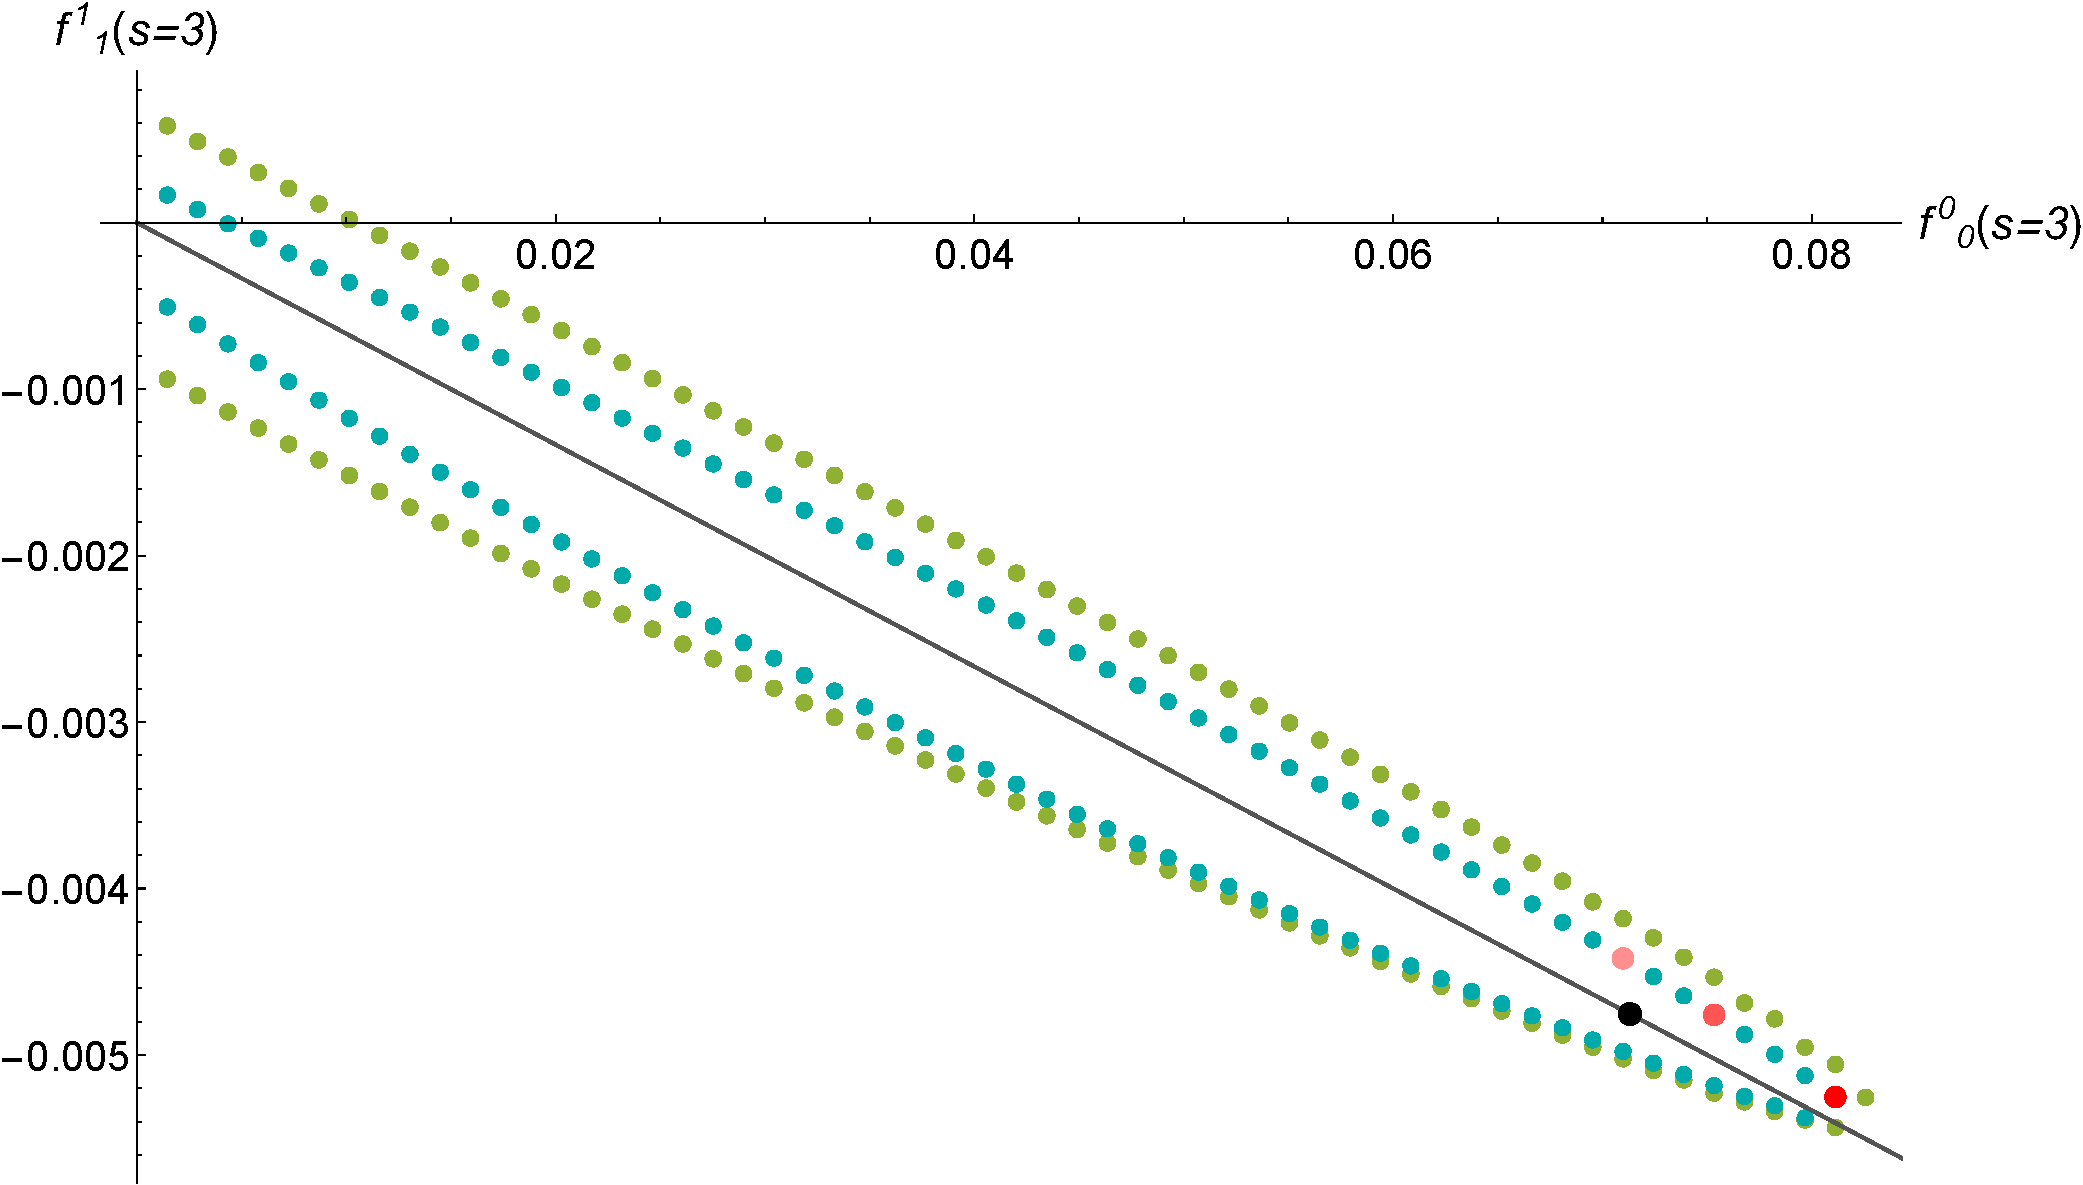
\includegraphics[width=.85\linewidth]{assets/original_chiSRplot.pdf}\end{center}
\begin{center}{\bfseries 当前同模型 IR／UV 对照}\\[1mm]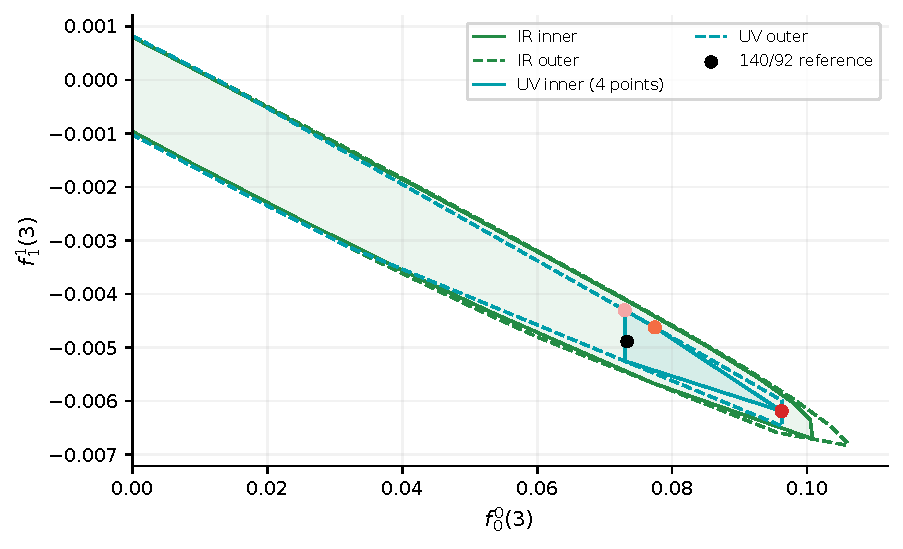
\includegraphics[width=.85\linewidth]{assets/ours_fig8.pdf}\end{center}
\boxnote{amber}{\textbf{已证：}UV右端及物理 \(x_{\rm ref}\) 处上下两侧都严格内缩。\\
\textbf{未复现：}原图明显更强的上侧收缩；本方上下比值约在 [0.9554,1.1803]。未填充的UV左侧不是已证明被排除的区域。}
\src{[1] Fig.8，PDF 第32页；[8] E1\_IR\_lower\_003、E1\_PAPER\_RESULT。}

\Ppage{E1--E2：支持界与三点的身份}{eselection}{给专家可核查的区间；选点规则先于相位}
\[
x_{\max}^{\rm UV}\le .096326220916201
<.10084542\le x_{\max}^{\rm IR}.
\]
后一个不等式使用同模型已验IR振幅，因此右端严格缩小不依赖继续细化所有区域方向。下表为便于阅读的舍入显示，严格区间端点见[8]的JSON证书。

{\small\begin{tabularx}{\linewidth}{@{}p{35mm}Y@{}}\toprule
\(x_{\rm ref}\) 截面&原式区间\\\midrule
IR 下／上边界&[-.00547303947,-.00545259192] ／ [-.00412892267,-.00411495563]\\
UV 下／上边界&[-.00527203156,-.00526642115] ／ [-.00432807821,-.00432632519]\\
上侧下降&[.00019740253,.00021312259]\\
下侧抬升&[.00018056036,.00020661832]\\
上／下变化之比&[.9553970459,1.1803398565]，跨1\\\bottomrule
\end{tabularx}}
原图约5.35来自显示标记凸包的截面读数，不是作者精确支持证书；但当前有效上限1.18034已说明，继续收紧此模型当前区间不能把它变成约5.35。

{\small\begin{tabularx}{\linewidth}{@{}p{13mm}p{42mm}p{36mm}Y@{}}\toprule
角色&预先固定的规则&保存投影约 \((x,y)\)&目标 gap\\\midrule
tip&完整 \(+x\) 支持&(.09622922,-.00618902)&\(9.6998\times10^{-5}\)\\
mid&固定 \(x=.07745128712\)，最大化 \(500y\)&(.07745129,-.00462509)&\(7.7053\times10^{-4}\)\\
ref&固定 \(x=.07298305468\)，最大化 \(500y\)&(.07298305,-.00430375)&\(7.6804\times10^{-4}\)\\\bottomrule
\end{tabularx}}
两个 near-black 的 x 由原Fig.8相对黑点的比例乘当前 \(x_{\rm ref}\) 得到。mid/ref 的 gap 是相应支持泛函的单位，不能当成 y 误差；实际 y 上侧距离分别不超过约 \(1.5411\times10^{-6}\)、\(1.5361\times10^{-6}\)。
\src{[3,8] PAPER\_MAINLINE、各 selection/report、Arb截面证书；完整4076维向量均保存。}

\Ppage{E3／Fig.9：QCD 输入后的 P1}{fig9}{原图与当前三代表点；两侧都含原论文的灰色实验／现象学参照}
\pairfig{original_P1ps.pdf}{ours_E_P1.pdf}{9}
\vspace{3mm}
\boxnote{teal}{\textbf{机制主张得到示例支持：}三点均有 \(90^\circ\) 上穿，区别于C的IR-only P1。没有在优化中使用770 MeV或实验相位作为目标。}
{\small\begin{tabularx}{\linewidth}{@{}p{14mm}p{40mm}p{28mm}p{23mm}Y@{}}\toprule
角色&原生括区（MeV）&线性读数（MeV）&相对770&P1最小 \(\eta\)\\\midrule
tip&[731.675,792.136]&788.621&+2.42\%&.630996\\
mid&[680.414,731.675]&700.403&-9.04\%&.387090\\
ref&[680.414,731.675]&696.267&-9.58\%&.237792\\\bottomrule
\end{tabularx}}
\boxnote{red}{\textbf{三点稳健性尚未复现：}读数跨度92.35 MeV；原Fig.9三条约812.5--826.6 MeV，跨度约14 MeV。仅“三条都有上穿”不足以宣称原论文的三点接近程度通过。}

\textbf{相移精度的独立信息：}最后两份已完成、原式通过的中心之间，P1最大模π相位变化为 tip .229°、mid .094°、ref .181°。该有限路径变化远小于主要三点差异，但仍不是到精确极值的统一相位误差界。

\textbf{读数性质：}这里是原生节点之间的描述性线性插值，不是复平面 \(\rho\) 极点质量。原生 \(S\) 决定相移模π，主图使用阈值锚定的 nearest-S 展开。
\src{[1] Fig.9，PDF 第33页；[8] E3\_PAPER\_RESULT、E3\_paper\_phases、E\_CENTER\_STABILITY。}

\Ppage{E3／Fig.10：S0、S2 原图对照}{fig10}{同一三套完整联合解；不是另选的 S 波最优解}
\pairfig{original_S0ps.pdf}{ours_E_S0.pdf}{10(a)：S0}
\vspace{5mm}
\pairfig{original_S2ps.pdf}{ours_E_S2.pdf}{10(b)：S2}
\vspace{3mm}
{\small\begin{tabularx}{\linewidth}{@{}p{29mm}YYY@{}}\toprule
同原生 \(s\) 的 RMS 差（度）&S0&S2&P1\\\midrule
tip&22.755&1.299&7.119\\
mid&11.523&2.098&25.093\\
ref&9.328&1.521&24.931\\\bottomrule
\end{tabularx}}
\boxnote{amber}{S2比较较接近；S0尤其tip的中高能与原图差异明显。P1中段差异也大，不能由约0.3\%的原图显示能标差消除。RMS是源图marker的描述性差值，不是统计误差。}
\src{[1] Fig.10，PDF 第34页；[8] E3\_paper\_comparison 的9组具名对照。}

\Ppage{电流 Gram、弹性程度与 Watson 机制}{eta}{论文给出物理论证；本页 \(\eta\) 是当前计算，没有对应原图 \(\eta\) 数据可逐点比较}
\begin{center}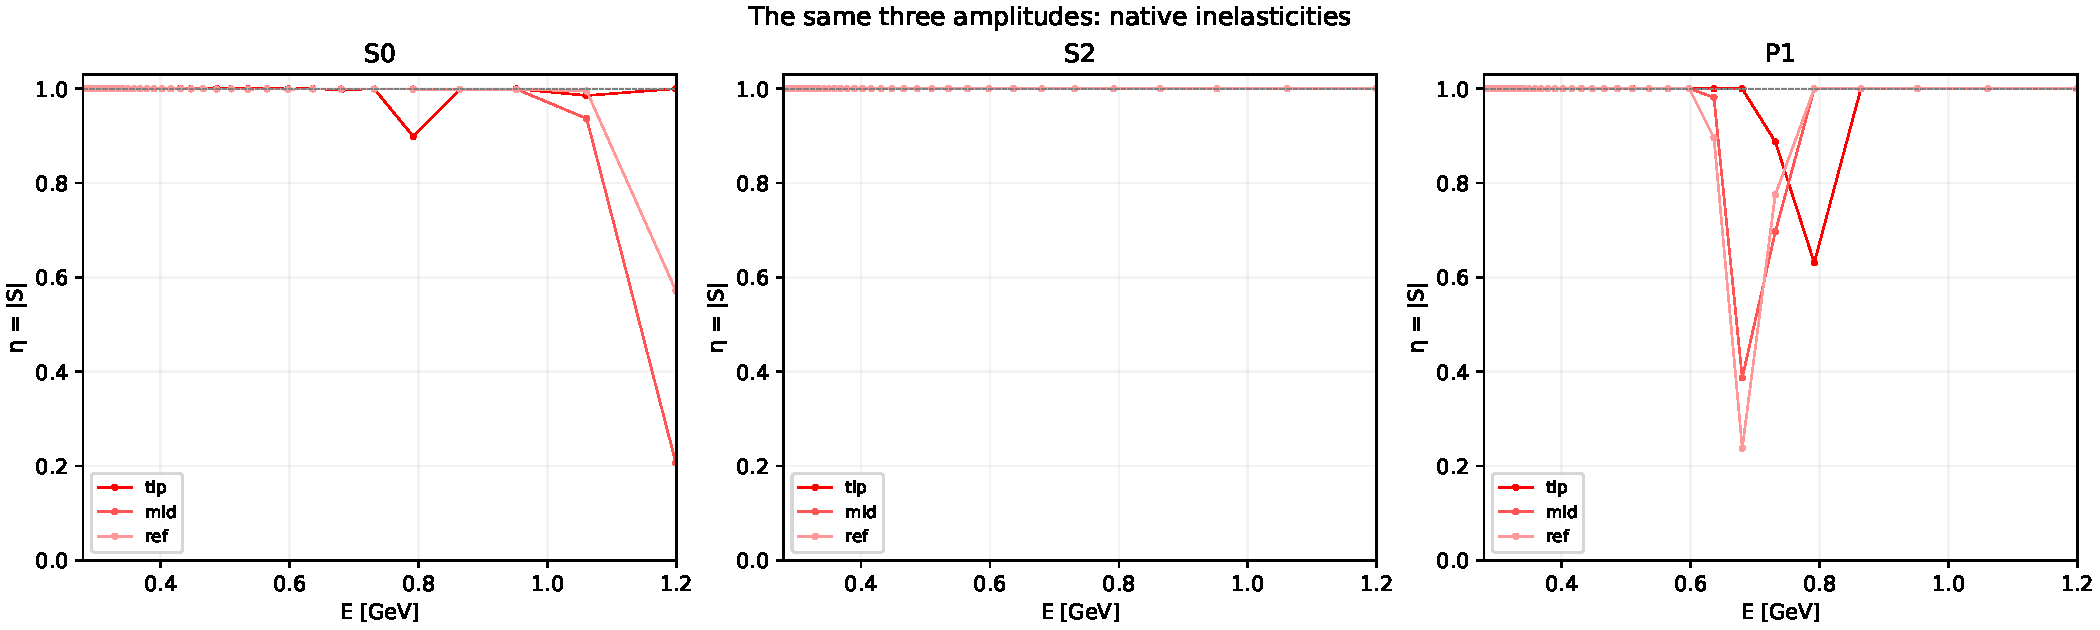
\includegraphics[width=\linewidth]{assets/ours_E_eta.pdf}\end{center}
\[
Q=\frac{F}{F^*},\quad F\ne0,\qquad
|S-Q|^2\le(1-|S|^2)\left(\frac{\rho_{\rm cur}}{|\mathcal F|^2}-1\right).
\]
这是原 Gram 行列式给出的精确后果。严格 \(\eta=1\)、非零F时，强制 \(S=Q\)。但当两 pion 谱份额 \(r=|\mathcal F|^2/\rho_{\rm cur}\) 很小时，\(\eta\) 数值上接近1本身不足以给出小的 Watson 相位误差。

\begin{tabularx}{\linewidth}{@{}p{23mm}YYY@{}}\toprule
当前三点&tip&mid&ref\\\midrule
S0 最小 \(\eta\)&.898599&.206946&.572231\\
P1 最小 \(\eta\)&.630996&.387090&.237792\\\bottomrule
\end{tabularx}
这些是被模型允许的非弹性，不是幺正盘的违例；却说明不能把原图的近弹性／谱饱和物理论证自动当作每个有限代表解都实现的性质。

\boxnote{amber}{\textbf{没有加入的额外物理条件：}没有强制所有点 \(\eta=1\)，没有强制 \(\rho_{\rm cur}=|\mathcal F|^2\)，也没有用 \(\arg[(S-1)/i]\) 替换主相位去改善图形。}
\textbf{相位分支：}FF引导的模π lift 仅是保留的条件诊断。它可保持同一S，却不能补出当前PV物理离节点的连续绕行、零点或极点证书。
\src{[2,4,8,11] SCIENCE、相位约定审计、原复Gram审计及当前诊断数据。}

\Ppage{F／Fig.11：论文原始五配置}{fig11original}{原图展示 \(M=50,L=8,10,12\) 与 \(L=10,M=45,50,60\)}
\begin{center}
{\small\bfseries S0}\\[-1mm]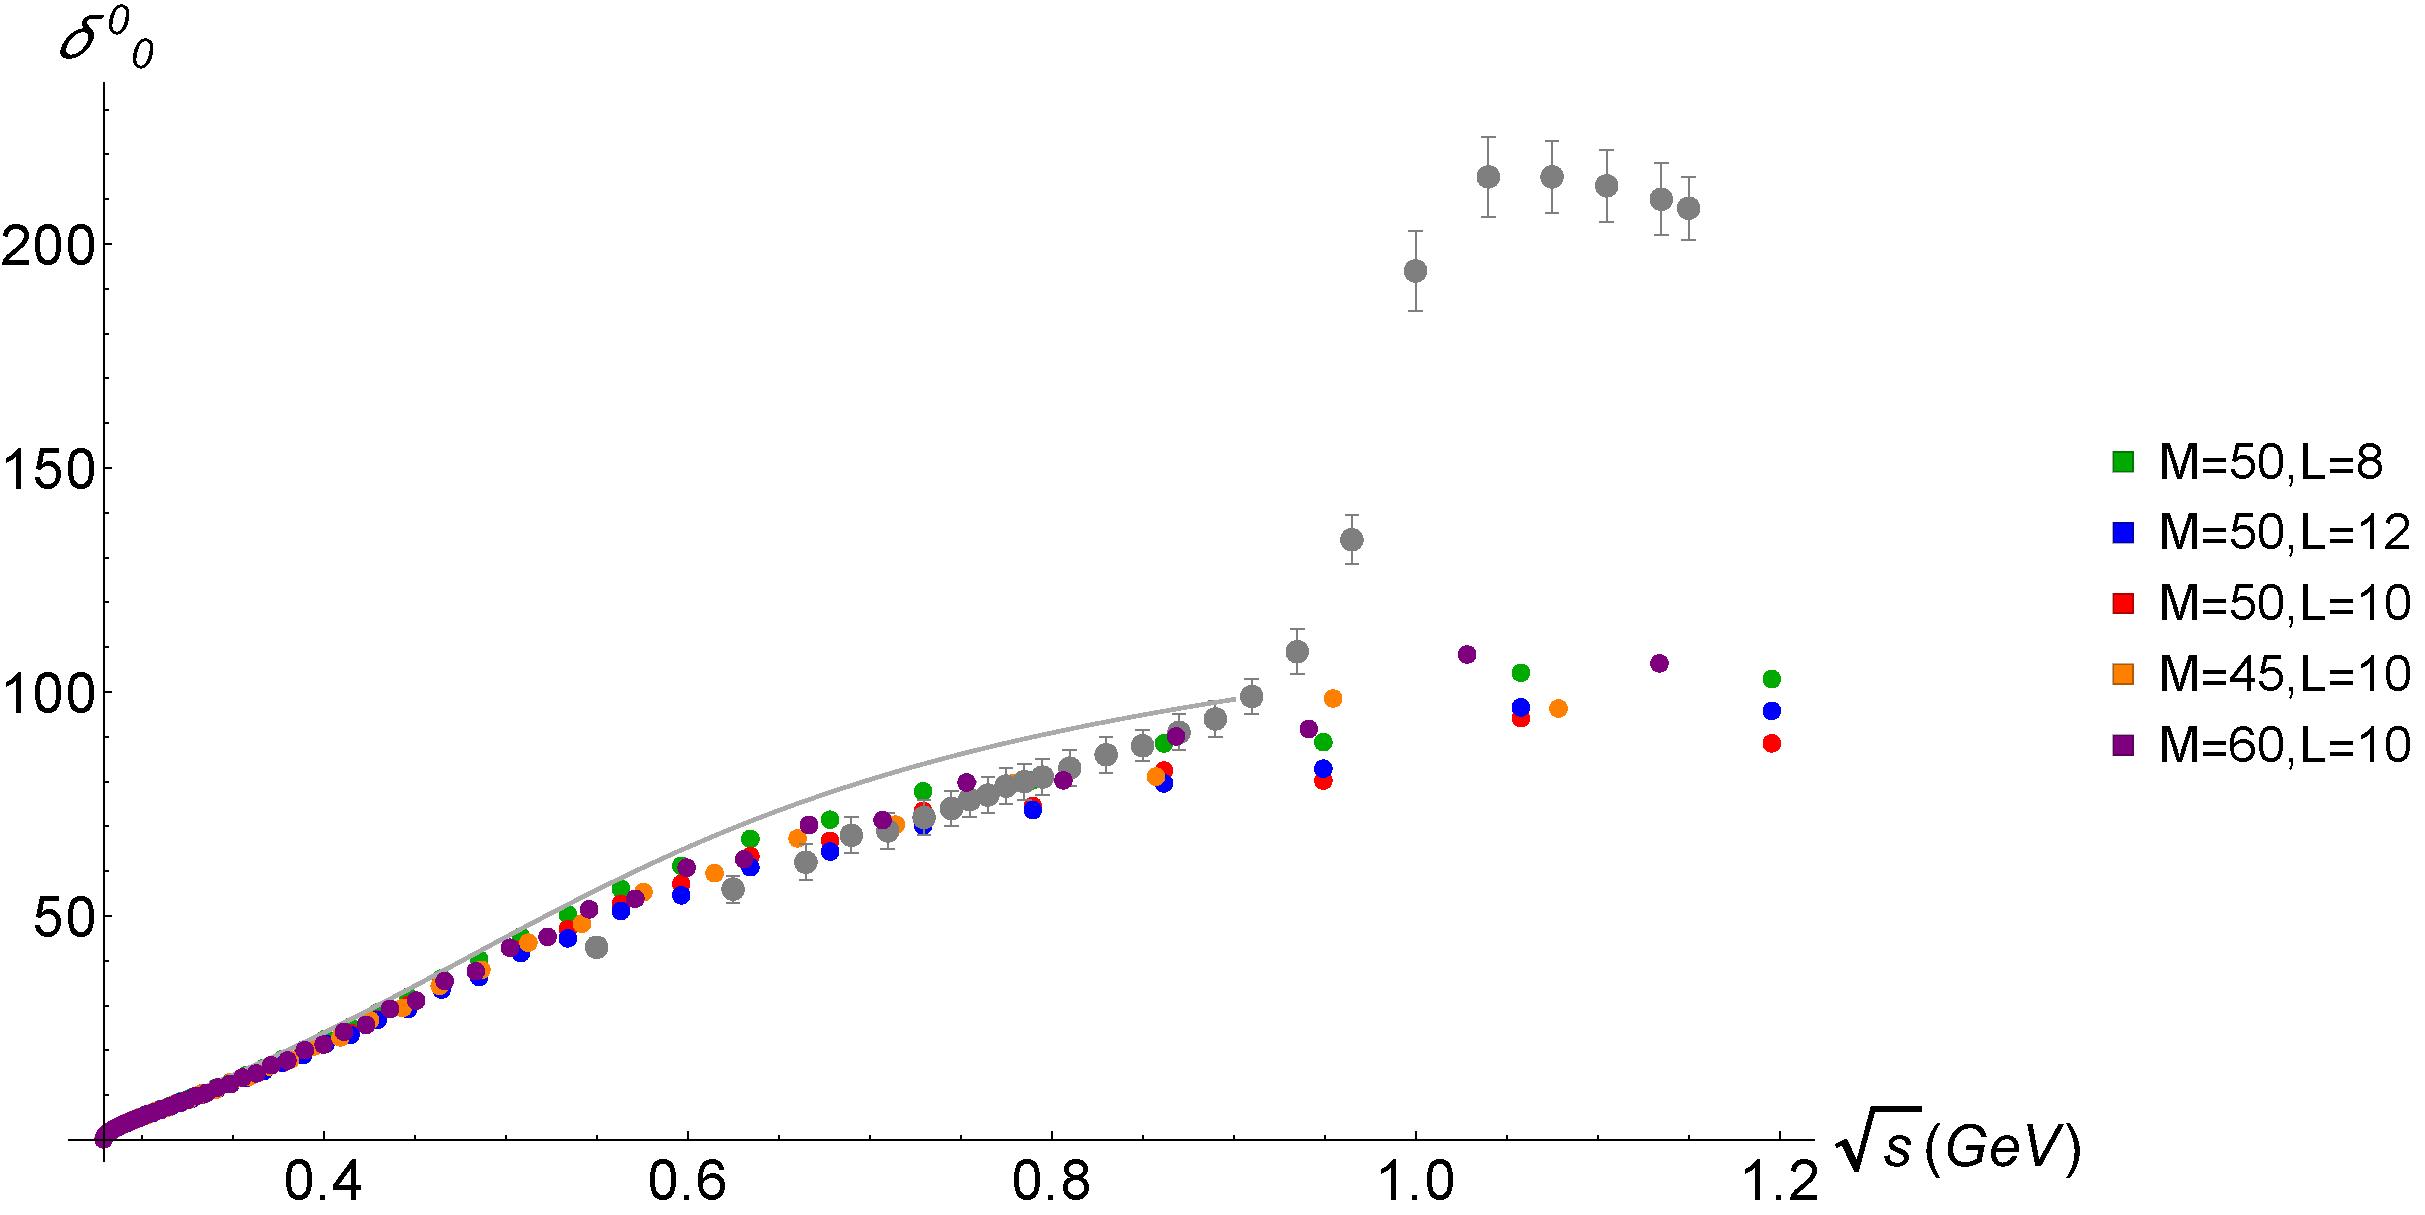
\includegraphics[width=.79\linewidth,height=60mm,keepaspectratio]{assets/original_S0ML.pdf}\\[2mm]
{\small\bfseries S2}\\[-1mm]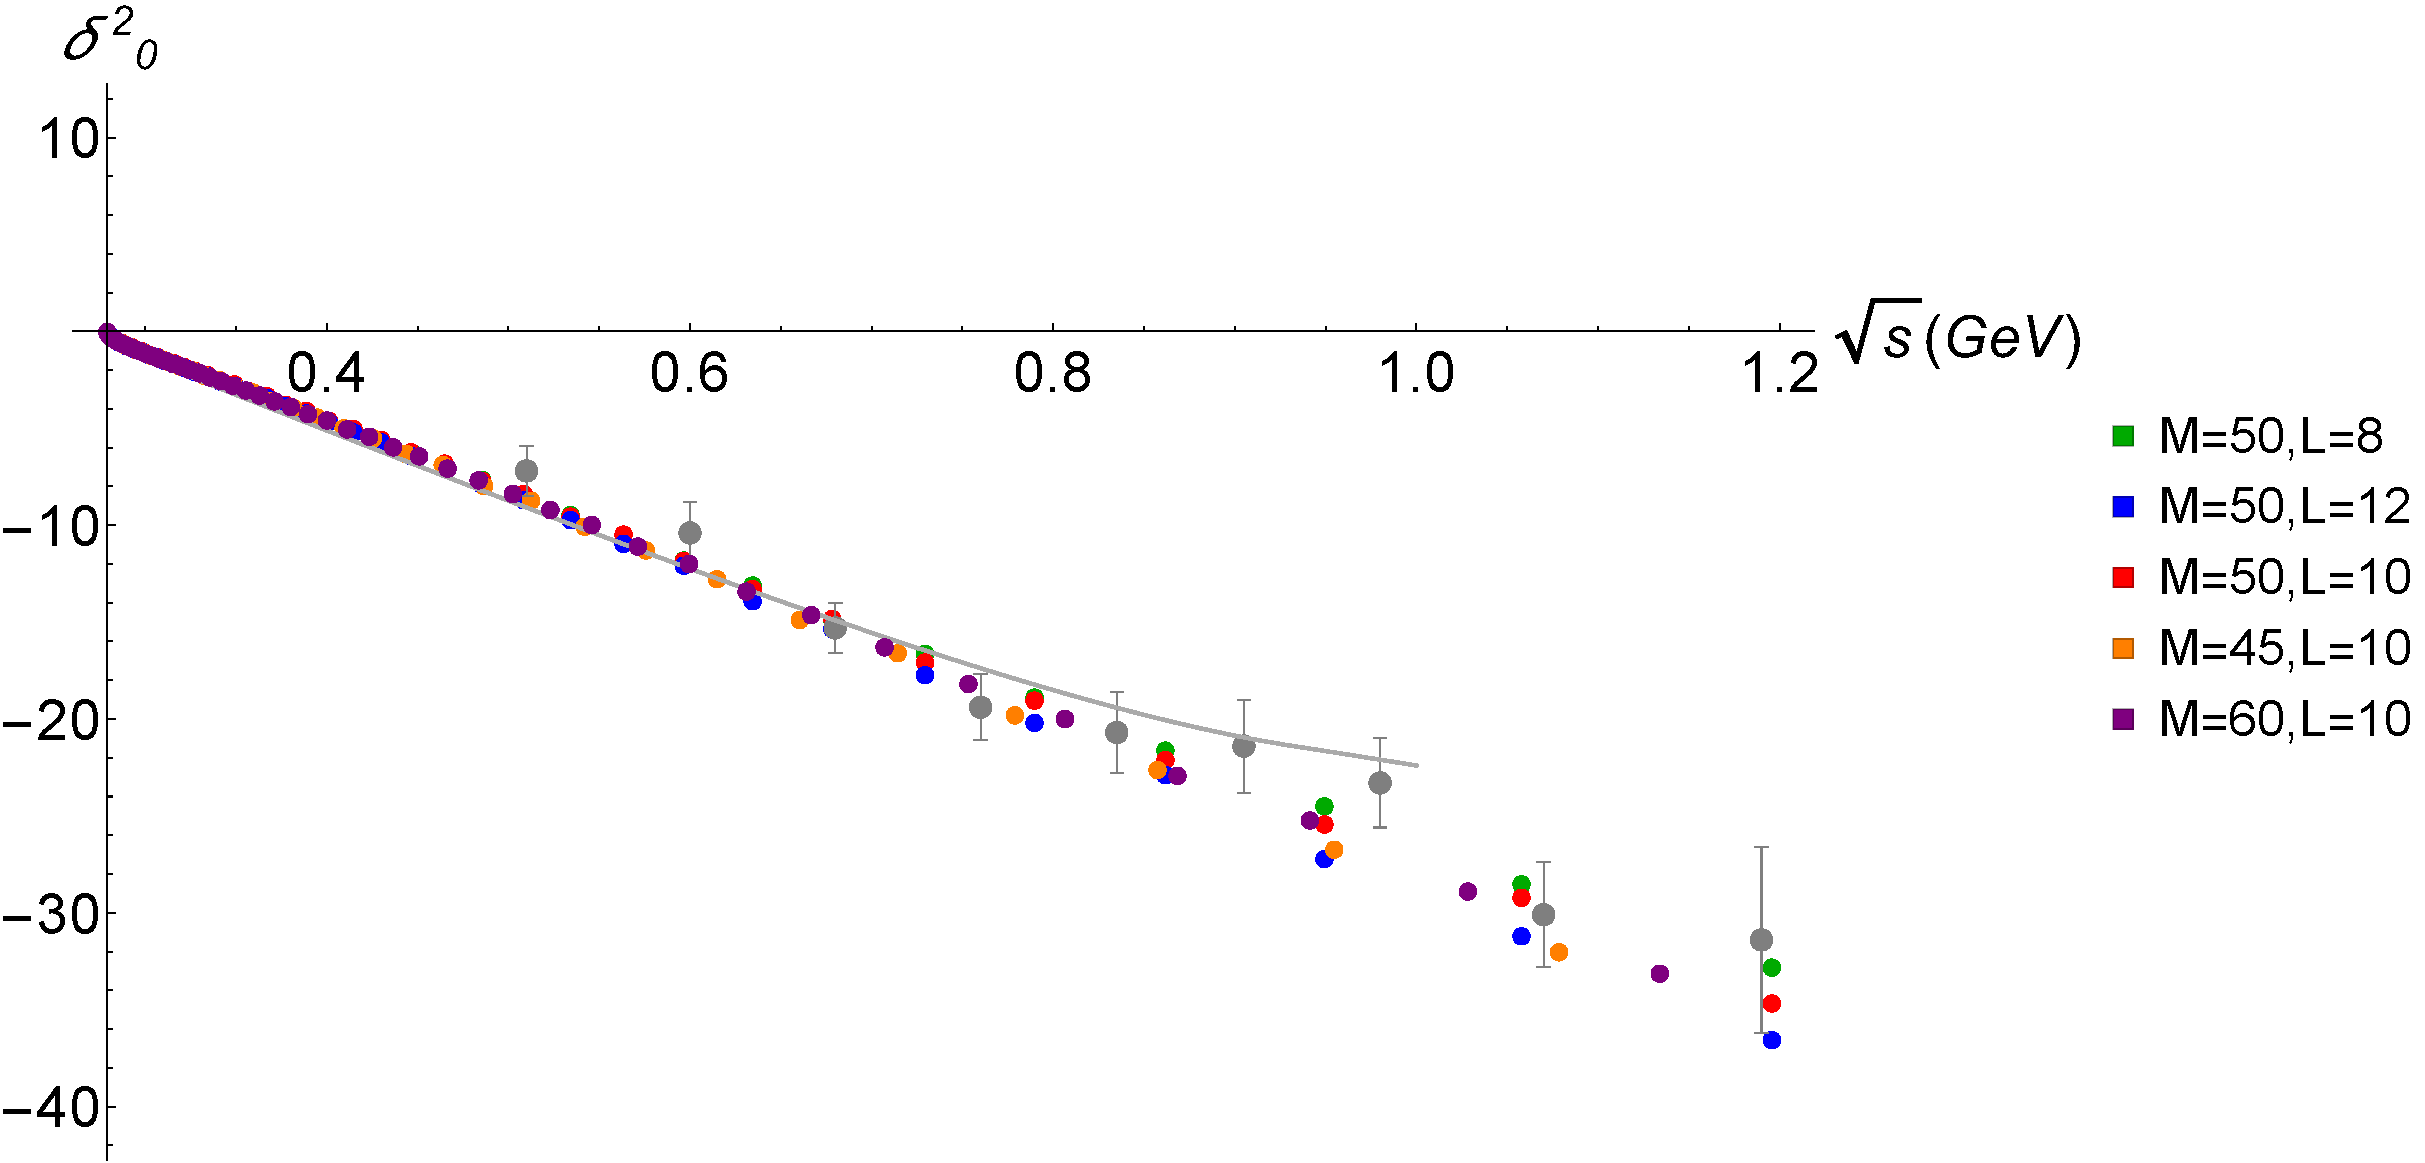
\includegraphics[width=.79\linewidth,height=60mm,keepaspectratio]{assets/original_S2ML.pdf}\\[2mm]
{\small\bfseries P1}\\[-1mm]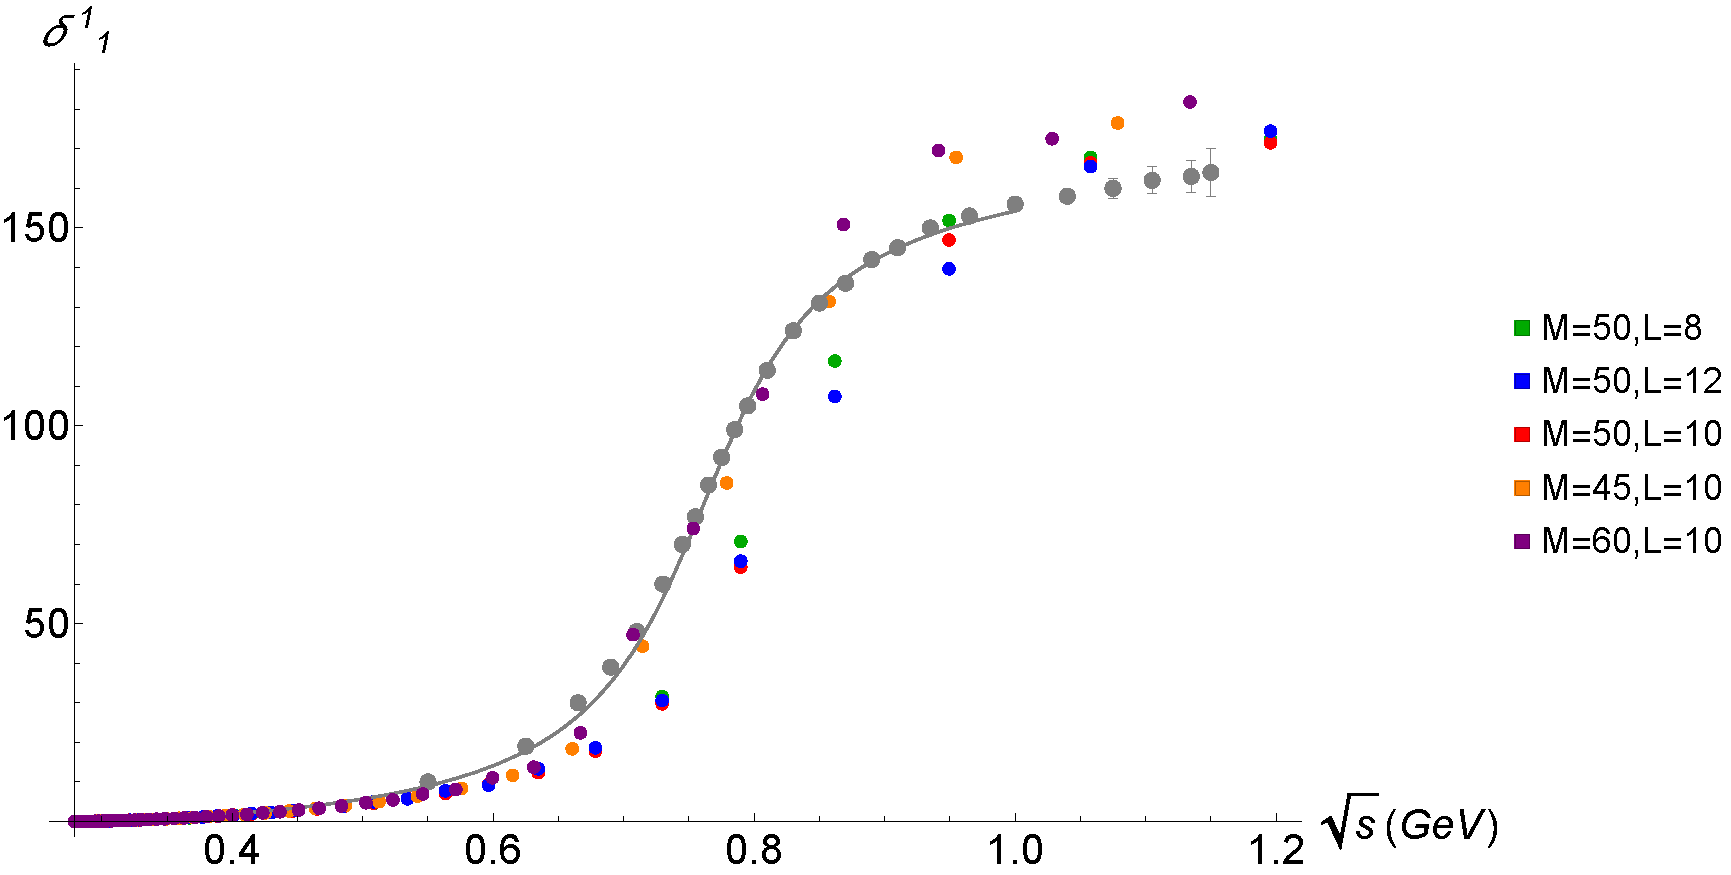
\includegraphics[width=.79\linewidth,height=60mm,keepaspectratio]{assets/original_P1ML.pdf}
\end{center}
\textbf{论文主张：}固定M改变L，三波有较好收敛；固定L改变M，S0/S2较稳定，P1的 \(\rho\) 仍出现而位置略变。作者指出改变M同时改变变量与幺正／SVZ约束，因此这不是只改变绘图密度。
\src{[1] Appendix A，Fig.11，PDF 第37页。三个面板直接来自原始 S0ML/S2ML/P1ML.pdf。}

\Ppage{F／Fig.11：当前四配置，明确缺 L12}{fig11ours}{左列固定M50仍不完整；右列固定L10的三M配置齐全}
\begin{center}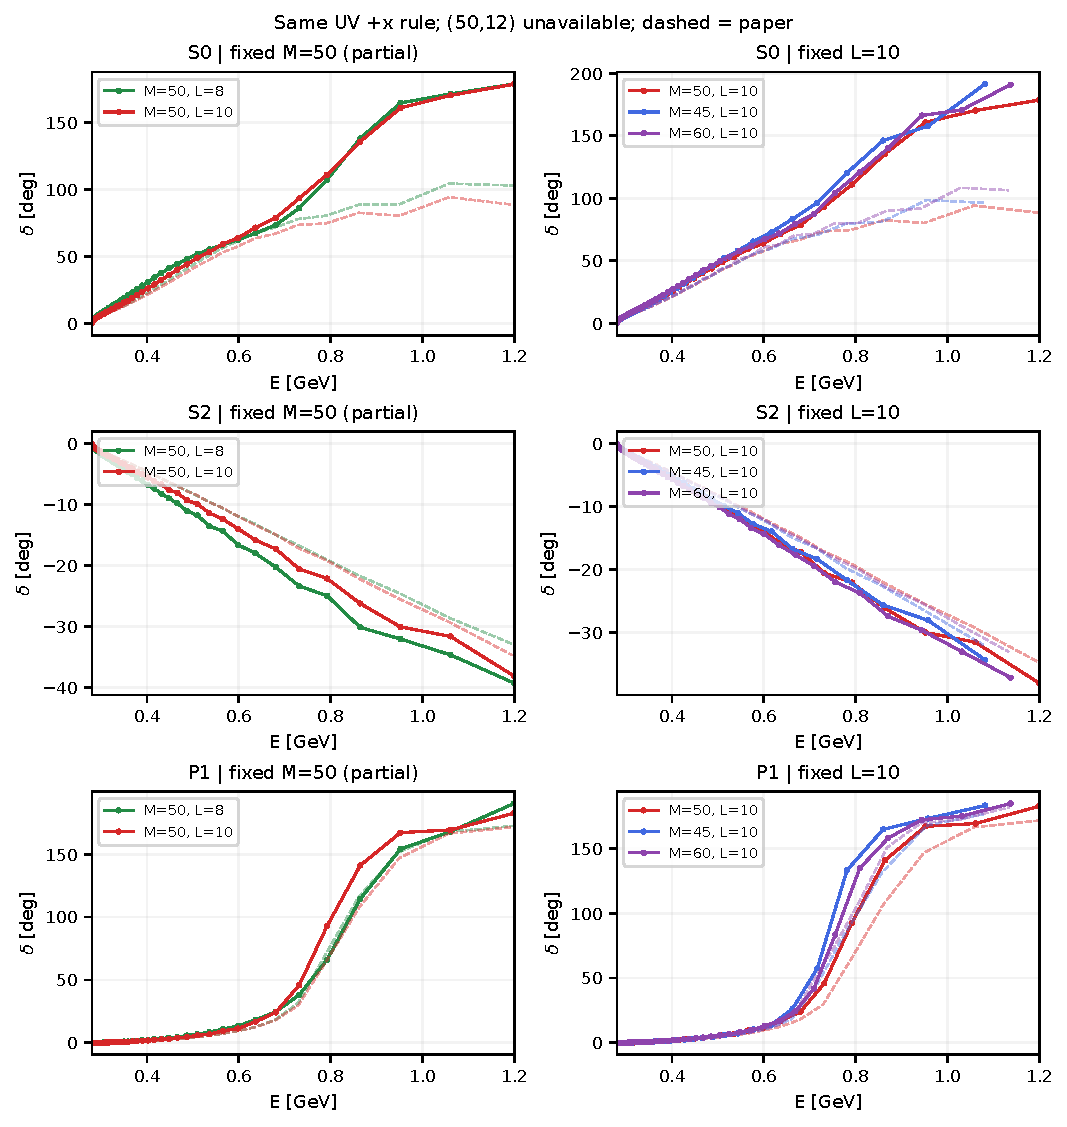
\includegraphics[width=.94\linewidth,height=175mm,keepaspectratio]{assets/ours_fig11_partial.pdf}\end{center}
{\small\begin{tabularx}{\linewidth}{@{}p{24mm}YYY@{}}\toprule
\((M,L)\)&原式支持gap&本次P1读数／MeV&原图读数／MeV\\\midrule
(50,8)&\(9.0652\times10^{-5}\)&828.015&820.117\\
(50,10)&\(9.6998\times10^{-5}\)&788.621&832.655\\
(45,10)&\(6.7980\times10^{-5}\)&744.342&786.551\\
(60,10)&\(8.0270\times10^{-5}\)&762.297&778.306\\\bottomrule
\end{tabularx}}
\src{[9] F\_paper/fig11\_partial。四个完整+x解均先固定后求相移；不以四组替代原文五组完成。}

\Ppage{F：稳定性证据与 L12 的真正缺口}{fquant}{配置齐全不自动等于收敛；求解失败不自动等于理论不可行}
\textbf{已完成部分。}四组均保留 \(\rho\) 式上穿。固定 L10 的三个M读数跨度44.28 MeV，原图约54.35 MeV，支持共振在这三种能量分辨率下保留。已完成的L8/L10就相差39.39 MeV，大于原图三个L约12.54 MeV的跨度；缺少L12不能隐藏这一已知差异。

\textbf{原式范围。}四组共5850个散射盘、410个电流Gram、4个χ球、4个密度界、16个FESR、60个FF界通过；另有537项原生主波求值通过。新图保留中高能S0差异。固定L的 \code{complete=true} 只表示三配置已齐，不代表所有物理主张已通过。

\begin{tabularx}{\linewidth}{@{}p{38mm}Y@{}}\toprule
L12 已执行的工作&结果与正确解释\\\midrule
L10中心向L12重验&新增高波盘真实违例；不能继承旧可行性。\\
同L12旧点／受限电流子问题&新χ／hard矩或联合Gram未过；受限失败不证明全空间不可行。\\
完整Phase I&全幅度方向开放，原散射／χ／L4保持硬；辅助 \(\tau\) 从约14.34降至 .05803。\\
最后同μ续算&仍未形成原联合见证；原零目标对偶界很松且为正，无不可行性证书。\\
代数恢复尝试&保旧四矩不保Gram；原Hermitian行列式出现严格负值，候选被拒绝。\\\bottomrule
\end{tabularx}
\boxnote{red}{\textbf{缺口不是仅有一个舍入末位：}最后候选有213个负Gram主子式，四个FESR余量均负，14个FF余量均负；最坏值分别约 \(-6.57\times10^{-4}\)、\(-1.16\times10^{-4}\)、\(-1.73\times10^{-6}\)。各类量单位不同，不能横向比较大小。微小χ回代超限另行记录，修复它不足以得到联合解。}
尚需同模型的有效联合见证（或真正不可行结论）；若可行，再做完整+x支持及相移。当前已停止重复追加同类迭代，\textbf{既没有宣称F完成，也没有宣称论文理论有缺陷}。
\src{[9] F\_RESULT、F\_PAPER\_PROGRESS、M50\_L12\_phase\_I\_08及代数复用反例。}

\Ppage{历史变体与具名后续方法}{history}{保留已有实现／失败的科学范围；不与当前模型拼成“全通过”}
\begin{tabularx}{\linewidth}{@{}p{34mm}Y@{}}\toprule
变体&已有工作及当前定位\\\midrule
separate-L2／clipped&历史B六域和E/F计算已交付；范数、截止改变后，不继承为当前模型的可行／最优证书。\\
hard／separate-L2&曾取得共同见证与部分支持，现仅作来源／数值对照。\\
finite-sine／FG／尾部&解析、秩及必要条件证据保留；活跃执行退休，不转移到PV连续性质。\\
2403 Watsonian&代码仍保留具名目标及数值诊断；不是2309已公开的原始算法，当前F协议没有加入。\\\bottomrule
\end{tabularx}
后续方法从上一完整解构造 \(Q=F_{\rm old}/F_{\rm old}^*\)（S0/P1），S2使用旧S，优化
\[
W=\frac1{3N_{\rm low}}\sum_{I,j}\Lambda_\ell(s_j)^{-2}
\operatorname{Re}\!\left[Q_{Ij}^*(S^{\rm new}_{Ij}-1)\right],
\quad \Lambda_0=1,\quad \Lambda_1=\frac{\sqrt{s-4}}{\sqrt s+2}.
\]
全部原物理约束保留；按作者后续做法释放原投影等式，因此新点必须记录移动后的坐标。完成一次固定旧Q的优化不等于新S/F已达固定点。
\begin{center}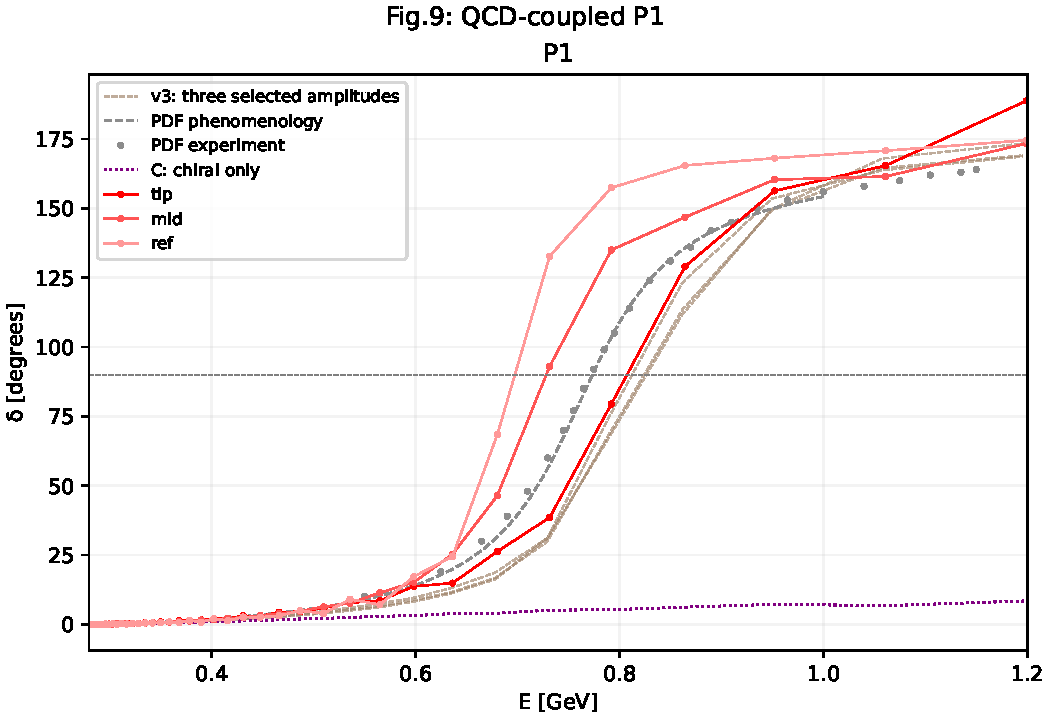
\includegraphics[width=.85\linewidth,height=65mm,keepaspectratio]{assets/historical_W_fig9.pdf}\end{center}
上图是\textbf{历史 separate／clipped 模型}的一次 Watsonian 结果。tip、mid、ref 读数约807.57、728.39、697.60 MeV，跨度约110 MeV。它展示可执行的后续步骤，\textbf{不能代替当前三点或证明2309全部claims完成}。
\src{[12] 2403.10772v4 Eq.(2.29)及作者代码；历史 stage\_E\_closure\_20260909/E3\_W\_phases。}

\Ppage{缺陷分类与需要专家判断的问题}{limits}{先区分来源、算法与物理结果，再决定下一项计算}
\begin{tabularx}{\linewidth}{@{}p{27mm}Yp{39mm}@{}}\toprule
问题类型&当前具体缺口&不能用什么替代\\\midrule
原设置身份&2309原始producer未公开；B正则化、完整散射处方、SR误差尺度／分组、精确选点尚未唯一恢复。&不能扫参数贴原图。\\
有限数值求解&B3整体精度未完成；F12尚无新共同见证，也无不可行证书。&不能把超时或正τ当定理。\\
已算物理差异&E1强非对称、E三点ρ接近程度、中高能S0与部分L稳定性仍不匹配。&不能只提高bits或gap后宣布消失。\\
连续物理范围&PV没有完整物理离节点延拓；无限能量／无限自旋未认证。&不能把更多有限样本说成全域证明。\\\bottomrule
\end{tabularx}

\textbf{建议专家优先判断的四个问题}
\begin{enumerate}
\item 现有公开资料是否足以唯一规定2309的有限数值问题？还需要原作者哪些矩阵、正则化、SR归一化与选点信息？
\item 当前PV节点／离切线的组合与原文方法是否达到了预期原型层面的对齐？哪些连续性质只能作为后续工作？
\item 在不改变物理集合的前提下，是否应先建立同一H／电流算子的MOSEK对照，以判定F12数值瓶颈？不能预设它一定更快或一定产生原图。
\item 哪些已经得到支持的机制主张可以报告，哪些稳定性或定量主张应明确保留为未复现？
\end{enumerate}
\boxnote{amber}{\textbf{本项目当前的审慎表述：}未在已核对的归一化、角投影、实际ρ打包、Gram共轭及FESR/FF单位中发现需直接修正的重大错误；这不等于排除了所有实现错误，更不等于全部原始数值设置已恢复。}
\textbf{推进边界：}没有为了得到原图而放宽幺正性、强制弹性、输入 \(\rho\) 质量、逐点改相位分支或隐去失败。下一步应由上面可区分的问题驱动，而非继续无限时间的同类试算。

\Ppage{代码、运行接口与随 PDF 附件}{codepage}{十个活跃模块；全部主要计算共用一个入口}
{\small\begin{tabularx}{\linewidth}{@{}p{31mm}Y@{}}\toprule
文件&当前科学职责\\\midrule
\code{__init__}&公共类型、数值运输、共同结果序列化\\
\code{model}&物理归一化、电流算子、观测量及原图比较\\
\code{kernels}&独立PV振幅、解析核、联合原式审计\\
\code{operators}&网格／算子、联合状态、分辨率运输\\
\code{imaginary}&散射支持编排、原式外界、PSD工具\\
\code{linear}&B/E完整Newton与CG求解\\
\code{quotient}&密度障碍、FESR目标、换元、B对偶、D初始化\\
\code{analysis}&C/E选点、区域／相移、Phase I启动\\
\code{io}&区域记录、Fig.3--11和η图\\
\code{run}&统一CLI与联合计算派发\\\bottomrule
\end{tabularx}}
十文件合计3317行、241494字节，各自不超过350行／24KiB；三个测试文件。重构后79项检查通过。18项关键数学／循环比较保持一致；报告组装与模块职责发生归并，未以数量限制删除物理变量或约束。

\begin{quote}\small\ttfamily
python -m smatrix\_bootstrap.run \textit{command} ...\\
prepare / prepare-current / boundary / dual / evaluate\\
regions / select / profiles / gauge-regions / select-gauge\\
gauge-phases / resolution / compare
\end{quote}
\textbf{典型数据链：}prepare输出H；D加入current算子；boundary输出完整系数／joint与界；evaluate恢复原生波；compare／resolution从保存的数据作原图与分辨率比较。原式支持不会由绘图或测试状态自动补齐。

\boxnote{teal}{\textbf{PDF附件 \code{reproduction_supplement.zip}：}包含当前十个核心文件、三个测试、项目配置、STATUS/SCIENCE/运行指南、当前输入合同、主要结果说明与小型曲线／汇总数据。附件可在支持附件的PDF阅读器中提取。}
大型H／current算子、全部中间日志与历史证明producer不重复嵌入本PDF；它们的仓库路径在下一页列明。附件代码是报告日期的快照，不包含未公开的2309原作者程序。
\src{[11] core10\_review：79测试、数学比对、接口与退休清单、原M50联合界及1500原生分波复核。}

\Ppage{来源索引与可重查路径}{sources}{原论文页码均指本地43页PDF的物理页；本文数字来自相应保存记录}
{\small
\begin{enumerate}[label={[\arabic*]},leftmargin=2em,itemsep=4pt]
\item Y. He, M. Kruczenski, \textit{Bootstrapping gauge theories}, \href{https://arxiv.org/abs/2309.12402v3}{arXiv:2309.12402v3}。本地 \code{references/2309.12402v3.pdf}；原图资产在 \code{references/2309.12402v3-source/}。
\item \code{STATUS.md}、\code{SCIENCE.md}、\code{REPRODUCTION_GUIDE_ZH.md}：本次汇报使用的当前状态与方法合同。
\item \R\code{PAPER_MAINLINE.json}：输入、范数、截止与相位前选点。
\item 同一R目录：\code{CHIRAL_SOURCE_RESIDUALS_ZH.md}、\code{CUTOFF_DECISION_ZH.md}、\code{NORMALIZATION_TRANSFER_ZH.md}、\code{PHASE_CONVENTION_DECISION_ZH.md}。
\item \R\code{B_combined/FIG4_CORE_CLAIMS_ZH.md}；\code{B_combined/regions_IR_lower_003/regions.json}及\code{comparisons.json}。共同H：\code{results/runs/stage_B_pv_M50_L10_prepare_20260907/}。
\item \R\code{C_RESULT_ZH.md}；\code{C1_fig5/}、\code{C2_fig6/}、\code{C3_fig7/}、\code{C_comparison/}。原图读数：\code{references/figure5_subthreshold.csv}及具名phase参考。
\item \R\code{D_RESULT_ZH.md}；\code{D1_hard_M50/}、\code{D3_paper_hull/}。完整维数与原式结果取最新report。
\item \R\code{E1_PAPER_RESULT_ZH.md}、\code{E3_PAPER_RESULT_ZH.md}、\code{E1_IR_lower_003/}、\code{E3_paper_phases/}、\code{E3_paper_comparison/}；三点为\code{paper_tip_path_02/}、\code{paper_mid_path_03/}、\code{paper_ref_path_02/}。
\item \R\code{F_paper/F_RESULT_ZH.md}、\code{F_paper/F_PAPER_PROGRESS_ZH.md}、\code{F_paper/fig11_partial/}、\code{F_paper/curve_comparison/}。L12末状态：\code{F_paper/M50_L12_phase_I_08/}；缺项没有计入五组通过。
\item \R\code{SOLVER_DECISION_ZH.md}、\code{B_SOLVER_FIX_ZH.md}。官方方法说明：\href{https://docs.mosek.com/latest/pythonapi/solving-conic.html}{MOSEK conic interior-point}，\href{https://clarabel.org/stable/}{Clarabel}。
\item 独立数学审计：\code{results/runs/stage_E_closure_audit_20260909/OPERATOR_AUDIT_ZH.md}。当前R目录：\code{core10_review/verification.json}、\code{core10_joint_audit/}、\code{core10_fresh_native/}。历史完整代码／测试：\code{results/evidence/core_before_ten_modules_20260910.json.gz}。
\item 作者后续工作 \href{https://arxiv.org/abs/2403.10772}{2403.10772v4} 与 \href{https://arxiv.org/abs/2505.19332}{2505.19332}；\href{https://github.com/hyfysics/gauge-theory-bootstrap}{官方代码仓库}。本文只援引具名方法和源码证据，不将后续整套输入冒充2309。
\end{enumerate}}
\boxnote{navy}{\textbf{给专家的最终状态：}当前报告可支持“有限原型与原式核验链已实现，IR/UV机制比较有实算证据”；尚不能支持“2309全部主张、全部原图身份及连续物理性质均已复现”。}
\end{document}
